\documentclass[]{tufte-book}

% ams
\usepackage{amssymb,amsmath}

\usepackage{ifxetex,ifluatex}
\usepackage{fixltx2e} % provides \textsubscript
\ifnum 0\ifxetex 1\fi\ifluatex 1\fi=0 % if pdftex
  \usepackage[T1]{fontenc}
  \usepackage[utf8]{inputenc}
\else % if luatex or xelatex
  \makeatletter
  \@ifpackageloaded{fontspec}{}{\usepackage{fontspec}}
  \makeatother
  \defaultfontfeatures{Ligatures=TeX,Scale=MatchLowercase}
  \makeatletter
  \@ifpackageloaded{soul}{
     \renewcommand\allcapsspacing[1]{{\addfontfeature{LetterSpace=15}#1}}
     \renewcommand\smallcapsspacing[1]{{\addfontfeature{LetterSpace=10}#1}}
   }{}
  \makeatother

\fi

% graphix
\usepackage{graphicx}
\setkeys{Gin}{width=\linewidth,totalheight=\textheight,keepaspectratio}

% booktabs
\usepackage{booktabs}

% url
\usepackage{url}

% hyperref
\usepackage{hyperref}

% units.
\usepackage{units}


\setcounter{secnumdepth}{2}

% citations

% pandoc syntax highlighting
\usepackage{color}
\usepackage{fancyvrb}
\newcommand{\VerbBar}{|}
\newcommand{\VERB}{\Verb[commandchars=\\\{\}]}
\DefineVerbatimEnvironment{Highlighting}{Verbatim}{commandchars=\\\{\}}
% Add ',fontsize=\small' for more characters per line
\newenvironment{Shaded}{}{}
\newcommand{\KeywordTok}[1]{\textcolor[rgb]{0.00,0.44,0.13}{\textbf{#1}}}
\newcommand{\DataTypeTok}[1]{\textcolor[rgb]{0.56,0.13,0.00}{#1}}
\newcommand{\DecValTok}[1]{\textcolor[rgb]{0.25,0.63,0.44}{#1}}
\newcommand{\BaseNTok}[1]{\textcolor[rgb]{0.25,0.63,0.44}{#1}}
\newcommand{\FloatTok}[1]{\textcolor[rgb]{0.25,0.63,0.44}{#1}}
\newcommand{\ConstantTok}[1]{\textcolor[rgb]{0.53,0.00,0.00}{#1}}
\newcommand{\CharTok}[1]{\textcolor[rgb]{0.25,0.44,0.63}{#1}}
\newcommand{\SpecialCharTok}[1]{\textcolor[rgb]{0.25,0.44,0.63}{#1}}
\newcommand{\StringTok}[1]{\textcolor[rgb]{0.25,0.44,0.63}{#1}}
\newcommand{\VerbatimStringTok}[1]{\textcolor[rgb]{0.25,0.44,0.63}{#1}}
\newcommand{\SpecialStringTok}[1]{\textcolor[rgb]{0.73,0.40,0.53}{#1}}
\newcommand{\ImportTok}[1]{#1}
\newcommand{\CommentTok}[1]{\textcolor[rgb]{0.38,0.63,0.69}{\textit{#1}}}
\newcommand{\DocumentationTok}[1]{\textcolor[rgb]{0.73,0.13,0.13}{\textit{#1}}}
\newcommand{\AnnotationTok}[1]{\textcolor[rgb]{0.38,0.63,0.69}{\textbf{\textit{#1}}}}
\newcommand{\CommentVarTok}[1]{\textcolor[rgb]{0.38,0.63,0.69}{\textbf{\textit{#1}}}}
\newcommand{\OtherTok}[1]{\textcolor[rgb]{0.00,0.44,0.13}{#1}}
\newcommand{\FunctionTok}[1]{\textcolor[rgb]{0.02,0.16,0.49}{#1}}
\newcommand{\VariableTok}[1]{\textcolor[rgb]{0.10,0.09,0.49}{#1}}
\newcommand{\ControlFlowTok}[1]{\textcolor[rgb]{0.00,0.44,0.13}{\textbf{#1}}}
\newcommand{\OperatorTok}[1]{\textcolor[rgb]{0.40,0.40,0.40}{#1}}
\newcommand{\BuiltInTok}[1]{#1}
\newcommand{\ExtensionTok}[1]{#1}
\newcommand{\PreprocessorTok}[1]{\textcolor[rgb]{0.74,0.48,0.00}{#1}}
\newcommand{\AttributeTok}[1]{\textcolor[rgb]{0.49,0.56,0.16}{#1}}
\newcommand{\RegionMarkerTok}[1]{#1}
\newcommand{\InformationTok}[1]{\textcolor[rgb]{0.38,0.63,0.69}{\textbf{\textit{#1}}}}
\newcommand{\WarningTok}[1]{\textcolor[rgb]{0.38,0.63,0.69}{\textbf{\textit{#1}}}}
\newcommand{\AlertTok}[1]{\textcolor[rgb]{1.00,0.00,0.00}{\textbf{#1}}}
\newcommand{\ErrorTok}[1]{\textcolor[rgb]{1.00,0.00,0.00}{\textbf{#1}}}
\newcommand{\NormalTok}[1]{#1}

% longtable
\usepackage{longtable,booktabs}

% multiplecol
\usepackage{multicol}

% strikeout
\usepackage[normalem]{ulem}

% morefloats
\usepackage{morefloats}


% tightlist macro required by pandoc >= 1.14
\providecommand{\tightlist}{%
  \setlength{\itemsep}{0pt}\setlength{\parskip}{0pt}}

% title / author / date
\title{Cleaning \& Transformation Tutorial}
\author{Gert Janssenswillen}
\date{}


\begin{document}

\maketitle



{
\setcounter{tocdepth}{1}
\tableofcontents
}

\begin{verbatim}
## Last updated on 2019-03-18
\end{verbatim}

\chapter*{Before you start}\label{before-you-start}
\addcontentsline{toc}{chapter}{Before you start}

During this tutorial, we'll use several r-packages. Make sure to install
and load them, if needed.

\begin{Shaded}
\begin{Highlighting}[]
\KeywordTok{library}\NormalTok{(ggplot2)}
\KeywordTok{library}\NormalTok{(dplyr)}
\KeywordTok{library}\NormalTok{(forcats)}
\KeywordTok{library}\NormalTok{(mice)}
\end{Highlighting}
\end{Shaded}

The \texttt{forcats} package contains a series of functions to easily
manipulate factors (of which \emph{forcats} is an anagram). The
\texttt{mice} package can be used to analyze the occurence of missing
values (\emph{MICE} stands for \emph{Multiple Imputation by Chained
Equations}, refering to a technique to estimate missing values).

We also assume that you are familiar with the content of both our
\texttt{ggplot2} and \texttt{dplyr} tutorial. You can read the
survey\footnote{The \texttt{survey} data used comes from the General
  Social Survey, and contains general information about social aspects
  of the American citizens. In particular, the \texttt{survey}
  data.frame contains a sample of categorical attributes.} dataset
provided with this tutorial if you want to try things out
yourself.\footnote{If you want to try things yourself, make sure to
  follow the tutorial step by step. The incremental nature of the
  cleaning and transformation process does not allow to perform parts of
  this tutorial in isolation.}

\begin{Shaded}
\begin{Highlighting}[]
\NormalTok{survey <-}\StringTok{ }\KeywordTok{readRDS}\NormalTok{(}\StringTok{"survey.RDS"}\NormalTok{)}
\KeywordTok{glimpse}\NormalTok{(survey)}
\end{Highlighting}
\end{Shaded}

\begin{verbatim}
## Observations: 21,483
## Variables: 9
## $ year    <chr> "2000", "2000", "2000", ...
## $ marital <chr> "Never married", "Divorc...
## $ age     <chr> "26", "48", "67", "39", ...
## $ race    <chr> "White", "White", "White...
## $ rincome <chr> "$8000 to 9999", "$8000 ...
## $ partyid <chr> "Ind,near rep", "Not str...
## $ relig   <chr> "Protestant", "Protestan...
## $ denom   <chr> "Southern baptist", "Bap...
## $ tvhours <chr> "12", NA, "2", "4", "1",...
\end{verbatim}

\chapter*{Introduction}\label{introduction}
\addcontentsline{toc}{chapter}{Introduction}

This tutorial on cleaning and transformation is divided into three
different sections.

\begin{itemize}
\tightlist
\item
  Reading
\item
  Cleaning
\item
  Transforming
\end{itemize}

\textbf{Reading}. The first task is to read the data provided in a
particular format into R. While we will not cover this topic
exhaustively, we will give useful pointers to appropriate R-packages to
do so.

\textbf{Cleaning}. We \emph{clean} the data by: removing mistakes,
duplicates, etc.

\textbf{Transforming}. Here we do not target the removal of mistakes and
inconsistencies, but rather try to make the data easier to analyse:
creating discrete representations of continuous variables, adding
calculated variables, or recoding the labels of categorical variables.

These steps in general take place before we do any of the analysis or
visualizations which we saw in the ggplot2 and dplyr tutorials, although
often multiple iterations are needed. Until now, we always received our
data in a fairly clean state, but that is rarely the case in reality.
Now, it's time to do our own cleaning. Let's go ahead!

\chapter{Reading data}\label{reading-data}

For our purpose, we will not discuss different data formats and how to
read them at length. \footnote{The section on reading data should be
  seen as background material for when you need it. You are only
  expected to be familiar with the functions and formats discussion in
  the classes. However, if you need to import a particular data file in
  your future career, you can use this as a starting point. The contents
  of this section can therefore partly skipped, \textbf{except} for the
  part on converting variables.} Mostly we will use the \texttt{readRDS}
function, which you probably have seen before. For example,

\begin{Shaded}
\begin{Highlighting}[]
\NormalTok{survey <-}\StringTok{ }\KeywordTok{readRDS}\NormalTok{(}\StringTok{"survey.RDS"}\NormalTok{)}
\end{Highlighting}
\end{Shaded}

A .RDS-file stores a \textbf{single} R-object in a serialized way. (RDS
can be thought of a R Data Serialized). We can create an .RDS-file using
\texttt{saveRDS} and read one using \texttt{readRDS}. Information
systems will \textbf{never} export data as .RDS files -- all .RDS-files
are created within R. All the .RDS-files you have been using in the
exercises and tutorials have been prepared by us. So, in which type of
files can data be found in the wild? Let's give you a quick tour of
common file formats.

\section{CSV and TSV}\label{csv-and-tsv}

CSV-files are probably thé most common type of data files. CSV stand for
Comma Seperated Values. These files can be seen as ordinary text files,
where each line is an observation, i.e.~a row, and columns are separated
with commas (therefore its name). The first row can contain the names of
the column, although this is not necessary. TSV is a much less common
variant, which stands for Tab Separated Values. As its name suggests,
values in this files are not seperated with commas but with tabs.

For CSV-files, there are two varying import functions: \texttt{read.csv}
and \texttt{read.csv2}. The first is for regular comma separated files,
while the latter is for semicolon seperated files. Otherwise, the usage
is similar to \texttt{readRDS}. The functions for TSV are similar --
just with a T instead of a C.

\begin{Shaded}
\begin{Highlighting}[]
\NormalTok{data <-}\StringTok{ }\KeywordTok{read.csv}\NormalTok{(}\StringTok{"path/to/data/file.csv"}\NormalTok{)}

\NormalTok{data <-}\StringTok{ }\KeywordTok{read.csv2}\NormalTok{(}\StringTok{"path/to/data/file.csv"}\NormalTok{)}
\end{Highlighting}
\end{Shaded}

Both these functions are base-R function, and have many additional
arguments to fine-tune the resulting data.frame based on peculiarities
in the data file. However, the have become less used since the
\texttt{readr} package from the tidyverse introduced faster functions
which better defaults. These functions are \texttt{read\_csv} and
\texttt{read\_csv2}, i.e.~with an underscore instead of a period.

\section{Excel}\label{excel}

While we do not like Excel very much, many people unfortunately still
do. As such, it will be probable that you have to read an Excel file
sooner or later. Reading Excel files can be done using the special
\texttt{readxl} package. This package contains the \texttt{read\_excel}
function.

\begin{Shaded}
\begin{Highlighting}[]
\NormalTok{data <-}\StringTok{ }\KeywordTok{read_excel}\NormalTok{(}\StringTok{"path/to/excel/file.xlsx"}\NormalTok{)}
\end{Highlighting}
\end{Shaded}

Again, just like for csv, there are many additional arguments in
\texttt{read\_excel}. For example, you can set the sheet in the excel
file you want to read, you can configure the types of the variables, and
you can even specify a range in the excel file that you want to read,
i.e.~B3:G8.

\section{JSON and XML}\label{json-and-xml}

JSON - or JavaScript Object Notation - and XML - eXtensible Markup
Language - are much more complex data notations compared with CSV. We
will not discuss these formats here, but instead just mention the
packages you can use if you every encounter these types.

\begin{itemize}
\tightlist
\item
  For JSON, the most common R-package is \texttt{jsonlite}, which
  contains the \texttt{fromJSON} function.
\item
  For XML, multiple options exists, but we advise the \texttt{xml2}
  package. For \texttt{xml} files, there is not a single function, but
  you'll typically to combine many functions to get the data in the
  right format.
\end{itemize}

\section{Other statistical packages}\label{other-statistical-packages}

Sometimes you will need to read data which comes from other commercial
data analysis and statistical software used by less R-savvy co-workers.
Often you need this because the analysis at hand cannot be done by the
commercial packages and R needs to rescue you. In particular, files can
come from SPSS, STATA and SAS. For each of these files, the
\texttt{haven} package contains a read-function.

\begin{Shaded}
\begin{Highlighting}[]
\CommentTok{# SPSS}
\KeywordTok{read_spps}\NormalTok{(}\StringTok{"file"}\NormalTok{)}

\CommentTok{# Stata}
\KeywordTok{read_dta}\NormalTok{(}\StringTok{"file"}\NormalTok{)}

\CommentTok{# sas}
\KeywordTok{read_sas}\NormalTok{(}\StringTok{"file"}\NormalTok{)}
\end{Highlighting}
\end{Shaded}

\section{Databases}\label{databases}

Finally, it is also possible to analyse data which is stored in a
data.base. The way to go here will depend on the type of database. One
of the useful packages in \texttt{DBI}, but you will need a specific
databased backend, such as \texttt{RMySL}, \texttt{RSQLite},
\texttt{RPostgreSQL}). Also useful is \texttt{dbplyr}, which enables
many \texttt{dplyr} functions to be used directly on a data base, such
that heavy computations don't have to be done by your pc.

\section{Background material}\label{background-material}

You can find more information on data import in Chapter 11 of the
\href{https://r4ds.had.co.nz/data-import.html}{R for Data Science book},
and on the help pages of mentioned packages and functions.

\textbf{\textless{} This is the end of the optional reading data section
\textgreater{}}

\section{Converting variables}\label{converting-variables}

Often an integral part of reading data from files, is making sure that
all the variables in our data are correctly stored. Let factors be
factors, and numbers be numbers. So, let's have a look at the dataset.

\begin{Shaded}
\begin{Highlighting}[]
\KeywordTok{glimpse}\NormalTok{(survey)}
\end{Highlighting}
\end{Shaded}

\begin{verbatim}
## Observations: 21,483
## Variables: 9
## $ year    <chr> "2000", "2000", "2000", ...
## $ marital <chr> "Never married", "Divorc...
## $ age     <chr> "26", "48", "67", "39", ...
## $ race    <chr> "White", "White", "White...
## $ rincome <chr> "$8000 to 9999", "$8000 ...
## $ partyid <chr> "Ind,near rep", "Not str...
## $ relig   <chr> "Protestant", "Protestan...
## $ denom   <chr> "Southern baptist", "Bap...
## $ tvhours <chr> "12", NA, "2", "4", "1",...
\end{verbatim}

That does not seem very right. Due to some evil forces, all the
variables are stored as characters, which isn't really correct. The
\texttt{year} and \texttt{age} variables certainly should be numeric,
while \texttt{marital}, for example, is clearly a nominal variable, and
should this be stored as factor.

The type of variables can be changed with the following functions:
\footnote{Note that these conversions are not by default without danger.
  For example, a variable can only made numeric if all its values can be
  treated as numeric values. If it finds values which cannot be
  correctly converted, such as text, it will insert a missing value
  instead (NA, for Not Available, as we will see below). Insertions of
  NA's will always lead to a warning. Such a warning will generally
  alert you that you did something wrong (did you convert a wrong
  variable?) or that there are errors in the data.}

\begin{itemize}
\tightlist
\item
  \texttt{as.numeric} -\textgreater{} for numeric variables
\item
  \texttt{as.integer} -\textgreater{} for integer variables
\item
  \texttt{as.factor} -\textgreater{} for nominal variables
\item
  \texttt{as.ordered} -\textgreater{} for ordinal variables
\item
  \texttt{as.character} -\textgreater{} for character variables
\end{itemize}

In order to fix this, let's use an old acquaintance from \texttt{dplyr}:
\texttt{mutate}. We already learned that mutate can be used to add new
variables to a datasets, but we can just as well use it to
\emph{overwrite} existing ones.

\begin{Shaded}
\begin{Highlighting}[]
\NormalTok{survey }\OperatorTok\StringTok{ }\KeywordTok{mutate}\NormalTok{(}\DataTypeTok{year =} \KeywordTok{as.integer}\NormalTok{(year), }\DataTypeTok{marital =} \KeywordTok{as.factor}\NormalTok{(marital), }
    \DataTypeTok{age =} \KeywordTok{as.integer}\NormalTok{(age), }\DataTypeTok{race =} \KeywordTok{as.factor}\NormalTok{(race), }
    \DataTypeTok{rincome =} \KeywordTok{as.factor}\NormalTok{(rincome), }\DataTypeTok{partyid =} \KeywordTok{as.factor}\NormalTok{(partyid), }
    \DataTypeTok{relig =} \KeywordTok{as.factor}\NormalTok{(relig), }\DataTypeTok{denom =} \KeywordTok{as.factor}\NormalTok{(denom), }
    \DataTypeTok{tvhours =} \KeywordTok{as.numeric}\NormalTok{(tvhours)) }\OperatorTok\StringTok{ }\NormalTok{glimpse}
\end{Highlighting}
\end{Shaded}

\begin{verbatim}
## Observations: 21,483
## Variables: 9
## $ year    <int> 2000, 2000, 2000, 2000, ...
## $ marital <fct> Never married, Divorced,...
## $ age     <int> 26, 48, 67, 39, 25, 25, ...
## $ race    <fct> White, White, White, Whi...
## $ rincome <fct> $8000 to 9999, $8000 to ...
## $ partyid <fct> "Ind,near rep", "Not str...
## $ relig   <fct> Protestant, Protestant, ...
## $ denom   <fct> Southern baptist, Baptis...
## $ tvhours <dbl> 12, NA, 2, 4, 1, NA, 3, ...
\end{verbatim}

That already looks better! However, observe that we did not yet store
the result of our efforts. In fact, we want to use this opportunity to
give all variables an easy name and undestandable name. For this, we can
use the \texttt{rename} function. \texttt{rename} is a dplyr function
with a very clear task: renaming variables. You can use it by giving it
a list of new names connected to old names:
\texttt{new\_name\ =\ old\_name}.

\begin{Shaded}
\begin{Highlighting}[]
\NormalTok{survey }\OperatorTok\StringTok{ }\KeywordTok{mutate}\NormalTok{(}\DataTypeTok{year =} \KeywordTok{as.integer}\NormalTok{(year), }\DataTypeTok{marital =} \KeywordTok{as.factor}\NormalTok{(marital), }
    \DataTypeTok{age =} \KeywordTok{as.integer}\NormalTok{(age), }\DataTypeTok{race =} \KeywordTok{as.factor}\NormalTok{(race), }
    \DataTypeTok{rincome =} \KeywordTok{as.factor}\NormalTok{(rincome), }\DataTypeTok{partyid =} \KeywordTok{as.factor}\NormalTok{(partyid), }
    \DataTypeTok{relig =} \KeywordTok{as.factor}\NormalTok{(relig), }\DataTypeTok{denom =} \KeywordTok{as.factor}\NormalTok{(denom), }
    \DataTypeTok{tvhours =} \KeywordTok{as.numeric}\NormalTok{(tvhours)) }\OperatorTok\StringTok{ }\KeywordTok{rename}\NormalTok{(}\DataTypeTok{reported_income =}\NormalTok{ rincome, }
    \DataTypeTok{party =}\NormalTok{ partyid, }\DataTypeTok{religion =}\NormalTok{ relig, }\DataTypeTok{denomination =}\NormalTok{ denom, }
    \DataTypeTok{tv_hours =}\NormalTok{ tvhours) }\OperatorTok\StringTok{ }\NormalTok{glimpse}
\end{Highlighting}
\end{Shaded}

\begin{verbatim}
## Observations: 21,483
## Variables: 9
## $ year            <int> 2000, 2000, 2000...
## $ marital         <fct> Never married, D...
## $ age             <int> 26, 48, 67, 39, ...
## $ race            <fct> White, White, Wh...
## $ reported_income <fct> $8000 to 9999, $...
## $ party           <fct> "Ind,near rep", ...
## $ religion        <fct> Protestant, Prot...
## $ denomination    <fct> Southern baptist...
## $ tv_hours        <dbl> 12, NA, 2, 4, 1,...
\end{verbatim}

Certainly, there is no right answer in naming variables. Just make sure
their names are understandable, easy to use and somewhat uniformly
typesetted.

Furthermore, note that what we just did is not the only possible way.
For instance, we could also directly create the new variable names with
mutate, although we will have to remove the old names afterwards.

\begin{Shaded}
\begin{Highlighting}[]
\NormalTok{survey }\OperatorTok\StringTok{ }\KeywordTok{mutate}\NormalTok{(}\DataTypeTok{year =} \KeywordTok{as.numeric}\NormalTok{(year), }\DataTypeTok{marital =} \KeywordTok{as.factor}\NormalTok{(marital), }
    \DataTypeTok{age =} \KeywordTok{as.numeric}\NormalTok{(age), }\DataTypeTok{race =} \KeywordTok{as.factor}\NormalTok{(race), }
    \DataTypeTok{reported_income =} \KeywordTok{as.factor}\NormalTok{(rincome), }\DataTypeTok{party =} \KeywordTok{as.factor}\NormalTok{(partyid), }
    \DataTypeTok{religion =} \KeywordTok{as.factor}\NormalTok{(relig), }\DataTypeTok{denomination =} \KeywordTok{as.factor}\NormalTok{(denom), }
    \DataTypeTok{tv_hours =} \KeywordTok{as.numeric}\NormalTok{(tvhours)) }\OperatorTok\StringTok{ }\KeywordTok{select}\NormalTok{(}\OperatorTok{-}\NormalTok{rincome}\OperatorTok{:-}\NormalTok{tvhours) }\OperatorTok\StringTok{ }
\StringTok{    }\NormalTok{glimpse}
\end{Highlighting}
\end{Shaded}

\begin{verbatim}
## Observations: 21,483
## Variables: 9
## $ year            <dbl> 2000, 2000, 2000...
## $ marital         <fct> Never married, D...
## $ age             <dbl> 26, 48, 67, 39, ...
## $ race            <fct> White, White, Wh...
## $ reported_income <fct> $8000 to 9999, $...
## $ party           <fct> "Ind,near rep", ...
## $ religion        <fct> Protestant, Prot...
## $ denomination    <fct> Southern baptist...
## $ tv_hours        <dbl> 12, NA, 2, 4, 1,...
\end{verbatim}

The result is the same, but the code is slightly shorter. If you really
want to master this, you might be interested to know that there are
plenty variants on mutate which might make your life even more easier
(or confused).

\begin{itemize}
\tightlist
\item
  transmute: this will \textbf{only} keep the \emph{new} variables your
  list in it
\item
  mutate\_if: this will work in the same way as select\_if,
  e.g.~applying a function on a certain type of columns
\item
  mutate\_at: this will apply a function on a certain set of columns you
  specify.
\end{itemize}

Don't worry. You'll come a long way if you can use select, mutate and
rename. But don't be afraid to challenge yourself and check out the more
advanced stuff.

Now, let's continue. Before we do, we copy the last part of code, this
time storing the result again as \texttt{survey}, thereby overwriting
the old version. You can do this in two ways: either put
\texttt{survey\ \textless{}-} before the piece of code, or put
\texttt{-\textgreater{}\ survey} after the piece of code. Again, there
is no wrong or right way. Personally, I prefer the later option, as it
nicely fits our narrative we created with the
\texttt{\%\textgreater{}\%} symbol: we take a dataset, we perform some
steps, and then we store it.

\begin{Shaded}
\begin{Highlighting}[]
\NormalTok{survey <-}\StringTok{ }\NormalTok{survey }\OperatorTok\StringTok{ }\KeywordTok{mutate}\NormalTok{(}\DataTypeTok{year =} \KeywordTok{as.numeric}\NormalTok{(year), }
    \DataTypeTok{marital =} \KeywordTok{as.factor}\NormalTok{(marital), }\DataTypeTok{age =} \KeywordTok{as.numeric}\NormalTok{(age), }
    \DataTypeTok{race =} \KeywordTok{as.factor}\NormalTok{(race), }\DataTypeTok{reported_income =} \KeywordTok{as.ordered}\NormalTok{(rincome), }
    \DataTypeTok{party =} \KeywordTok{as.factor}\NormalTok{(partyid), }\DataTypeTok{religion =} \KeywordTok{as.factor}\NormalTok{(relig), }
    \DataTypeTok{denomination =} \KeywordTok{as.factor}\NormalTok{(denom), }\DataTypeTok{tv_hours =} \KeywordTok{as.numeric}\NormalTok{(tvhours)) }\OperatorTok\StringTok{ }
\StringTok{    }\KeywordTok{select}\NormalTok{(}\OperatorTok{-}\NormalTok{rincome}\OperatorTok{:-}\NormalTok{tvhours)}
\end{Highlighting}
\end{Shaded}

This is a good place to pay attention to work-flow aspects. Before,
during the analysis of data, different pieces of code rarely depended on
each other. For example, if we made graph A and then table B, both could
be made independent from each other. We never stored the results we
created to be used later (apart from a sample of data we sometimes
took.) However, now that we will be cleaning and transforming the data,
we will always update the data.frame, typically under the same name.
Indeed, we don't want to end up with a list of survey, survey2, survey3,
survey4, without remembering their differences. So, at each step, we
update the previous version of survey.

However, there is a risk. If we make a mistake, our data could be
broken. For example, if we erroneously converted race to numeric, the
as.numeric function will fail to do so and create a column full of NAs
instead. We can then quickly correct our mistake in the code, but this
won't bring the original race variable back -- it was gone the moment we
mistakenly converted it.

To right our wrongs, we will need to reload the data, and all the
transformations we already applied before. Just correcting the code is
no longer going to be sufficient, \textbf{we need to correct our data}.
When working in R Markdown, this is easiest done with the central button
in an R-chunk, as this will rerun all the previous R-chunks, bringing
our data in the state it was in before.

These dependencies in our workflow also mean that exercises will more
depend on each other, and we must always be sure to save our updated
data.frame. Not updating the data (or running the code) will be a
frequent source of errors later on. Be aware. (You are warned)

\chapter{Cleaning Data}\label{cleaning-data}

Now that we have imported the data and made sure that all the variables
at least have to appropriate type, it's time to start cleaning the data.
In particular, we will cover the following topics

\begin{itemize}
\tightlist
\item
  Duplicates observations
\item
  Cleaning of categorical variables
\item
  Cleaning of continuous variables
\item
  Checking Data inconstencies
\end{itemize}

Furthermore, we will also spend some time discussing missing values.
That's a lot of concepts to cover, so let's get started!

\section{Duplicates Removal}\label{duplicates-removal}

Sometimes, it might happen that some rows were accidently included
multiple times in the dataset. There is an easy way to find these, and
to remove them.

The \texttt{duplicated} function (a base R function), returns a logical
vector indicating duplicate rows in a dataset. The vector will have the
same length as the number of rows in the dataset, and will be
\texttt{TRUE} for rows which are not unique, and \texttt{FALSE}
otherwise.

\begin{Shaded}
\begin{Highlighting}[]
\NormalTok{survey }\OperatorTok\StringTok{ }\NormalTok{duplicated }\OperatorTok\StringTok{ }\NormalTok{summary}
\end{Highlighting}
\end{Shaded}

\begin{verbatim}
##    Mode   FALSE    TRUE 
## logical   21220     263
\end{verbatim}

It seems that there are 263 in our data which are not unique. We can
take a look at these by using the output of duplicated as an input of
filter.\footnote{Noticed the . within the \texttt{duplicated} function?
  The point has a special significance if used together with the piping
  symbol. Internally, it will be replaced with the input coming through
  the piping symbol. As such,
  \texttt{gss\_cat\ \%\textgreater{}\%\ filter(duplicated(.))} is equal
  to \texttt{filter(gss\_cat,\ duplicated(gss\_cat))}. It's very
  convenient if you need to refer to the piping input multiple times,
  not only as the first argument of the function.}

\begin{Shaded}
\begin{Highlighting}[]
\NormalTok{gss_cat }\OperatorTok\StringTok{ }\KeywordTok{filter}\NormalTok{(}\KeywordTok{duplicated}\NormalTok{(.))}
\end{Highlighting}
\end{Shaded}

\begin{verbatim}
## # A tibble: 263 x 9
##     year marital   age race  rincome partyid
##    <int> <fct>   <int> <fct> <fct>   <fct>  
##  1  2000 Married    48 White $25000~ Ind,ne~
##  2  2000 Never ~    39 Other $25000~ Not st~
##  3  2000 Married    36 Other $25000~ Not st~
##  4  2000 Never ~    30 White $25000~ Not st~
##  5  2000 Never ~    19 White $1000 ~ Not st~
##  6  2000 Married    47 White $25000~ Not st~
##  7  2000 Married    29 White $25000~ Indepe~
##  8  2000 Married    39 White $10000~ Not st~
##  9  2000 Widowed    80 White Not ap~ Strong~
## 10  2002 Married    43 White Not ap~ Indepe~
## # ... with 253 more rows, and 3 more
## #   variables: relig <fct>, denom <fct>,
## #   tvhours <int>
\end{verbatim}

Right now we selected the duplicate rows and we can have a look at them.
If we only want to retain the unique rows, we can add a !-symbol to
negate the selection.

\begin{Shaded}
\begin{Highlighting}[]
\NormalTok{survey }\OperatorTok\StringTok{ }\KeywordTok{filter}\NormalTok{(}\OperatorTok{!}\KeywordTok{duplicated}\NormalTok{(.))}
\end{Highlighting}
\end{Shaded}

\begin{verbatim}
## # A tibble: 21,220 x 9
##     year marital   age race  reported_income
##    <dbl> <fct>   <dbl> <fct> <ord>          
##  1  2000 Never ~    26 White $8000 to 9999  
##  2  2000 Divorc~    48 White $8000 to 9999  
##  3  2000 Widowed    67 White Not applicable 
##  4  2000 Never ~    39 White Not applicable 
##  5  2000 Divorc~    25 White Not applicable 
##  6  2000 Married    25 White $20000 - 24999 
##  7  2000 Never ~    36 White $25000 or more 
##  8  2000 Divorc~    44 White $7000 to 7999  
##  9  2000 Married    44 White $25000 or more 
## 10  2000 Married    47 White $25000 or more 
## # ... with 21,210 more rows, and 4 more
## #   variables: party <fct>, religion <fct>,
## #   denomination <fct>, tv_hours <dbl>
\end{verbatim}

However, this is a little bit verbose. Therefore, \texttt{dplyr}
contains a very handy short cut: the \texttt{distinct} function.

\begin{Shaded}
\begin{Highlighting}[]
\NormalTok{survey }\OperatorTok\StringTok{ }\NormalTok{distinct}
\end{Highlighting}
\end{Shaded}

\begin{verbatim}
## # A tibble: 21,220 x 9
##     year marital   age race  reported_income
##    <dbl> <fct>   <dbl> <fct> <ord>          
##  1  2000 Never ~    26 White $8000 to 9999  
##  2  2000 Divorc~    48 White $8000 to 9999  
##  3  2000 Widowed    67 White Not applicable 
##  4  2000 Never ~    39 White Not applicable 
##  5  2000 Divorc~    25 White Not applicable 
##  6  2000 Married    25 White $20000 - 24999 
##  7  2000 Never ~    36 White $25000 or more 
##  8  2000 Divorc~    44 White $7000 to 7999  
##  9  2000 Married    44 White $25000 or more 
## 10  2000 Married    47 White $25000 or more 
## # ... with 21,210 more rows, and 4 more
## #   variables: party <fct>, religion <fct>,
## #   denomination <fct>, tv_hours <dbl>
\end{verbatim}

Whether we want to remove duplicate rows or not really depends on the
data. In our cases, it is not at all surprising that some of these rows
are the same. It just happens that some people are very much alike: the
same age, income, religion etc.

However, it other cases, such duplicate rows would be impossible. For
instance, if there are variables which would per definition make each
row unique, such as a national id number. In such cases, duplicate rows
clearly need further consideration and removing them might be the right
solution. But for now, let's continue.

\section{Cleaning Categorical
Variables}\label{cleaning-categorical-variables}

For the cleaning of categorical variables, we consider the following
changes

\begin{itemize}
\tightlist
\item
  Recoding values
\item
  Reordering values
\end{itemize}

\subsection{Recode Categorical
Variables}\label{recode-categorical-variables}

Sometimes, categorical variables, i.e.~factors, have weird or even wrong
labels. In that case, we would like to \emph{recode} these values.
Finding wrong labels isn't always easy, and often these mistakes will
surface later during the analysis, in which case you have to take a step
back and correct them afterwards. Nonetheless, looking at frequency
tables in alphabetical order, or ordered from least to most frequent,
can point to some mistakes.\footnote{The \texttt{count} function used
  here is a \texttt{dplyr} short hand for
  \texttt{group\_by(party)\ \%\textgreater{}\%\ summarize(n\ =\ n())}.
  Feel free to use it to save your from a lot of typing. It also has a
  sort argument for sorting on descending frequencies. As such,
  \texttt{count(party,\ sort\ =\ T)} is equal to
  \texttt{group\_by(party)\ \%\textgreater{}\%\ summarize(n\ =\ n())\ \%\textgreater{}\%\ arrange(-n)}.
  However, be aware the \texttt{count} will remove the entire grouping
  of a data.frame afterward, unlike \texttt{summarize}.} Let's take the
party variable as an example.

\begin{Shaded}
\begin{Highlighting}[]
\NormalTok{survey }\OperatorTok\StringTok{ }\KeywordTok{count}\NormalTok{(party)}
\end{Highlighting}
\end{Shaded}

\begin{verbatim}
## # A tibble: 10 x 2
##    party                  n
##    <fct>              <int>
##  1 Don't know             1
##  2 Ind,near dem        2499
##  3 Ind,near rep        1791
##  4 Independent         4119
##  5 No answer            154
##  6 Not str democrat    3690
##  7 Not str republican  3032
##  8 Other party          393
##  9 Strong democrat     3490
## 10 Strong republican   2314
\end{verbatim}

While the values for party are not really wrong, they are not every
uniform: Str and Strong, Ind and Independent. Let's change them. We can
recode factor levels using the \texttt{fct\_recode} function from
forcats. As arguments, we need to say which variable to recode, and
which levels to changes.

\begin{Shaded}
\begin{Highlighting}[]
\NormalTok{data }\OperatorTok
\StringTok{    }\KeywordTok{mutate}\NormalTok{(}\OperatorTok{<}\NormalTok{factor_name}\OperatorTok{>}\StringTok{ }\ErrorTok{=}\StringTok{ }\KeywordTok{fct_recode}\NormalTok{(}\OperatorTok{<}\NormalTok{factor_name}\OperatorTok{>}\NormalTok{, }
                                      \StringTok{"<new_level1>"}\NormalTok{ =}\StringTok{ "<old_level1>"}\NormalTok{,}
                                      \StringTok{"<new_level2>"}\NormalTok{ =}\StringTok{ "<old_level2>"}\NormalTok{)}
\end{Highlighting}
\end{Shaded}

We can recode as many old levels into new levels as we want.
Furthermore, you can replace several old levels by the same new level.
Any level not mentioned will be left unchanged. Let's create some
uniformity in the political affiliations.

\begin{Shaded}
\begin{Highlighting}[]
\NormalTok{survey <-}\StringTok{ }\NormalTok{survey }\OperatorTok\StringTok{ }\KeywordTok{mutate}\NormalTok{(}\DataTypeTok{party =} \KeywordTok{fct_recode}\NormalTok{(party, }
    \StringTok{`}\DataTypeTok{Republican, strong}\StringTok{`}\NormalTok{ =}\StringTok{ "Strong republican"}\NormalTok{, }
    \StringTok{`}\DataTypeTok{Republican, weak}\StringTok{`}\NormalTok{ =}\StringTok{ "Not str republican"}\NormalTok{, }
    \StringTok{`}\DataTypeTok{Independent, near rep}\StringTok{`}\NormalTok{ =}\StringTok{ "Ind,near rep"}\NormalTok{, }
    \StringTok{`}\DataTypeTok{Independent, near dem}\StringTok{`}\NormalTok{ =}\StringTok{ "Ind,near dem"}\NormalTok{, }
    \StringTok{`}\DataTypeTok{Democrat, weak}\StringTok{`}\NormalTok{ =}\StringTok{ "Not str democrat"}\NormalTok{, }\StringTok{`}\DataTypeTok{Democrat, strong}\StringTok{`}\NormalTok{ =}\StringTok{ "Strong democrat"}\NormalTok{))}
\end{Highlighting}
\end{Shaded}

Don't forget to update the dataset!

\subsection{Reorder Categorical
Variables}\label{reorder-categorical-variables}

Another possibility, especially for ordinal factors, is that the values
are not really wrong, but they are in the wrong order. For instance,
take a look at the reported income.

\begin{Shaded}
\begin{Highlighting}[]
\NormalTok{survey }\OperatorTok\StringTok{ }\KeywordTok{count}\NormalTok{(reported_income)}
\end{Highlighting}
\end{Shaded}

\begin{verbatim}
## # A tibble: 16 x 2
##    reported_income     n
##    <ord>           <int>
##  1 $1000 to 2999     395
##  2 $10000 - 14999   1168
##  3 $15000 - 19999   1048
##  4 $20000 - 24999   1283
##  5 $25000 or more   7363
##  6 $3000 to 3999     276
##  7 $4000 to 4999     226
##  8 $5000 to 5999     227
##  9 $6000 to 6999     215
## 10 $7000 to 7999     188
## 11 $8000 to 9999     340
## 12 Don't know        267
## 13 Lt $1000          286
## 14 No answer         183
## 15 Not applicable   7043
## 16 Refused           975
\end{verbatim}

The value ``Lt \$1000'' - meaning Limited, or less than \$1000 - should
be shown first, but instead it is in the wrong place. Here, we need
another forcats function, namely \texttt{fct\_relevel}. This function
can be used in two different ways to put a level into a different place.

\textbf{Option 1}: Move one (or more) level(s) to the front

\begin{Shaded}
\begin{Highlighting}[]
\NormalTok{data }\OperatorTok\StringTok{ }\KeywordTok{mutate}\NormalTok{(}\DataTypeTok{factor_name =} \KeywordTok{fct_relevel}\NormalTok{(factor_name, }
    \StringTok{"level1_to_move"}\NormalTok{, }\StringTok{"level2_to move"}\NormalTok{, }\StringTok{"..."}\NormalTok{))}
\end{Highlighting}
\end{Shaded}

\textbf{Option 2}: Insert one (or more) level(s) after a number N of
levels

\begin{Shaded}
\begin{Highlighting}[]
\NormalTok{data }\OperatorTok\StringTok{ }\KeywordTok{mutate}\NormalTok{(}\DataTypeTok{factor_name =} \KeywordTok{fct_relevel}\NormalTok{(factor_name, }
    \StringTok{"level1_to_move"}\NormalTok{, }\StringTok{"level2_to move"}\NormalTok{, }\StringTok{"..."}\NormalTok{, }
    \DataTypeTok{after =}\NormalTok{ N))}
\end{Highlighting}
\end{Shaded}

So, let's move the LT \$1000 level to the first place.

\begin{Shaded}
\begin{Highlighting}[]
\NormalTok{survey <-}\StringTok{ }\NormalTok{survey }\OperatorTok\StringTok{ }\KeywordTok{mutate}\NormalTok{(}\DataTypeTok{reported_income =} \KeywordTok{fct_relevel}\NormalTok{(reported_income, }
    \StringTok{"Lt $1000"}\NormalTok{))}
\end{Highlighting}
\end{Shaded}

We can check the results by using count on the updated \texttt{survey}
data.frame.

\begin{Shaded}
\begin{Highlighting}[]
\NormalTok{survey }\OperatorTok\StringTok{ }\KeywordTok{count}\NormalTok{(reported_income)}
\end{Highlighting}
\end{Shaded}

\begin{verbatim}
## # A tibble: 16 x 2
##    reported_income     n
##    <ord>           <int>
##  1 Lt $1000          286
##  2 $1000 to 2999     395
##  3 $10000 - 14999   1168
##  4 $15000 - 19999   1048
##  5 $20000 - 24999   1283
##  6 $25000 or more   7363
##  7 $3000 to 3999     276
##  8 $4000 to 4999     226
##  9 $5000 to 5999     227
## 10 $6000 to 6999     215
## 11 $7000 to 7999     188
## 12 $8000 to 9999     340
## 13 Don't know        267
## 14 No answer         183
## 15 Not applicable   7043
## 16 Refused           975
\end{verbatim}

Changing the order of levels of a categorical variable is useful for
both nominal and ordinal data. For ordinal data, it is logical that we
want to order of the levels to be the correct one. But also for nominal
data we might want to change the order. For example, there are often
catch-all values such as ``Other'' or ``Various''. It is good practice
to treat these values differently compared to the regular values in a
nominal, by putting them last. As such, they will shown up on one end of
a graph or table, and not in between the other values. Let's take a look
at party.

\begin{Shaded}
\begin{Highlighting}[]
\NormalTok{survey }\OperatorTok\StringTok{ }\KeywordTok{count}\NormalTok{(party)}
\end{Highlighting}
\end{Shaded}

\begin{verbatim}
## # A tibble: 10 x 2
##    party                     n
##    <fct>                 <int>
##  1 Don't know                1
##  2 Independent, near dem  2499
##  3 Independent, near rep  1791
##  4 Independent            4119
##  5 No answer               154
##  6 Democrat, weak         3690
##  7 Republican, weak       3032
##  8 Other party             393
##  9 Democrat, strong       3490
## 10 Republican, strong     2314
\end{verbatim}

Deciding whether a factor is ordinal or not is not always that
straigthforward. If we look at the reported income, it is clear that
there is an order. However, we didn't define \texttt{party} as an
ordered factor. There is no ``best'' or ``superior'' political party, so
explicitly program this variable as a ordinal factor would be one bridge
too far -- we would have to decide which end of the political spectrum
is the ``lowest'' and which the ``highest''. However, this is somewhat
undesirable if we make graphs.

\begin{Shaded}
\begin{Highlighting}[]
\NormalTok{survey }\OperatorTok\StringTok{ }\KeywordTok{ggplot}\NormalTok{(}\KeywordTok{aes}\NormalTok{(party)) }\OperatorTok{+}\StringTok{ }\KeywordTok{geom_bar}\NormalTok{(}\DataTypeTok{fill =} \StringTok{"dodgerblue4"}\NormalTok{) }\OperatorTok{+}\StringTok{ }
\StringTok{    }\KeywordTok{theme_light}\NormalTok{() }\OperatorTok{+}\StringTok{ }\KeywordTok{theme}\NormalTok{(}\DataTypeTok{axis.text.x =} \KeywordTok{element_text}\NormalTok{(}\DataTypeTok{angle =} \DecValTok{45}\NormalTok{, }
    \DataTypeTok{hjust =} \DecValTok{1}\NormalTok{))}
\end{Highlighting}
\end{Shaded}

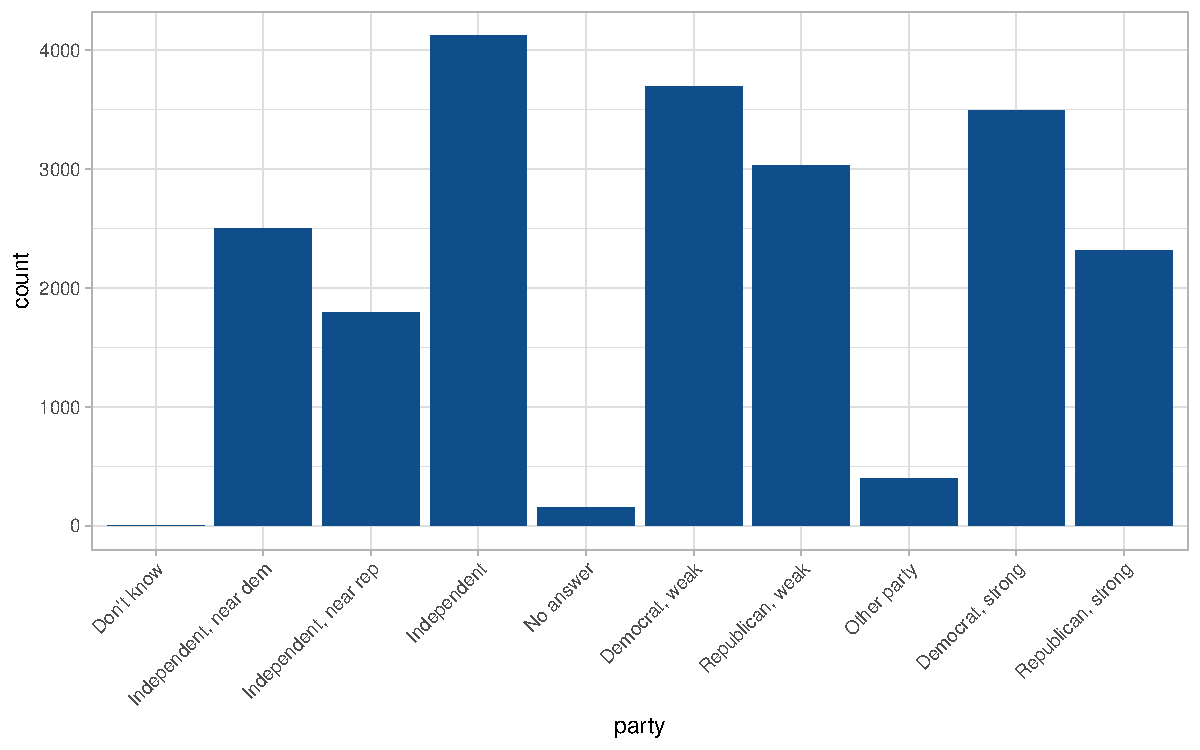
\includegraphics{cleaning_tutorial_files/figure-latex/unnamed-chunk-27-1}

When we don't have an ordinal factor, the order of labels will be often
be alphabetical. In this case, because we recoded the labels before,
they are not even in alphabetical order any more. \footnote{When we
  first did as.factor(party), the levels were placed in alphabetical
  order. However, we then recoded some levels, but this didn't update
  the order. Thus ``Strong Republican'' because ``Republican Strong''
  and ``Strong Democrate'' became ``Democrat Strong'', but both remained
  the last levels because they originally started with S. It's not
  expected that you are familiar with all the side-effects of some
  transformations, but this shows you the complexities when our actions
  start to depend on earlier actions, and how we are really working in
  an iterative context.}. The resulting graph is difficult to read, as
the x-axis is scrambled. A natural reflex would be to order the bar
chart according to frequency, but that would not really improve the
readability in this special case. Instead, we can apply a more logical
order, without necessary considering party as an ordinal variable. Such
a logical order is readily available for the current variable, as we
often speak of left and right-wing politics. We can leave the
alternative answers (Don't know, No Answer, Other Party), either at the
start or end of the order. By not noticing them in the code below, the
latter will happen.

\begin{Shaded}
\begin{Highlighting}[]
\NormalTok{survey <-}\StringTok{ }\NormalTok{survey }\OperatorTok\StringTok{ }\KeywordTok{mutate}\NormalTok{(}\DataTypeTok{party =} \KeywordTok{fct_relevel}\NormalTok{(party, }
    \StringTok{"Democrat, strong"}\NormalTok{, }\StringTok{"Democrat, weak"}\NormalTok{, }\StringTok{"Independent, near dem"}\NormalTok{, }
    \StringTok{"Independent"}\NormalTok{, }\StringTok{"Independent, near rep"}\NormalTok{, }\StringTok{"Republican, weak"}\NormalTok{, }
    \StringTok{"Republican, strong"}\NormalTok{))}
\end{Highlighting}
\end{Shaded}

Our graph now looks as follows. Better, isn't it? \footnote{Of course,
  \emph{better} is subjective and depends on what you like to show your
  audience. If the data would be about Flemish political parties, it's
  more difficult to apply a logical order. (I.e. who is more ``left'',
  Groen or Sp.a?) Because there are not the same nuances in these
  parties, such as ``weak'' or ``strong'', it would make more sense to
  order them according to frequencies. (Which is what happens in times
  of Flemish elections, but not necessarily in times of US elections.)
  In the end, none two situations are the same and much is left to your
  decisions and assumptions as data analyst.}

\begin{Shaded}
\begin{Highlighting}[]
\NormalTok{survey }\OperatorTok\StringTok{ }\KeywordTok{ggplot}\NormalTok{(}\KeywordTok{aes}\NormalTok{(party)) }\OperatorTok{+}\StringTok{ }\KeywordTok{geom_bar}\NormalTok{(}\DataTypeTok{fill =} \StringTok{"dodgerblue4"}\NormalTok{) }\OperatorTok{+}\StringTok{ }
\StringTok{    }\KeywordTok{theme_light}\NormalTok{() }\OperatorTok{+}\StringTok{ }\KeywordTok{theme}\NormalTok{(}\DataTypeTok{axis.text.x =} \KeywordTok{element_text}\NormalTok{(}\DataTypeTok{angle =} \DecValTok{45}\NormalTok{, }
    \DataTypeTok{hjust =} \DecValTok{1}\NormalTok{))}
\end{Highlighting}
\end{Shaded}

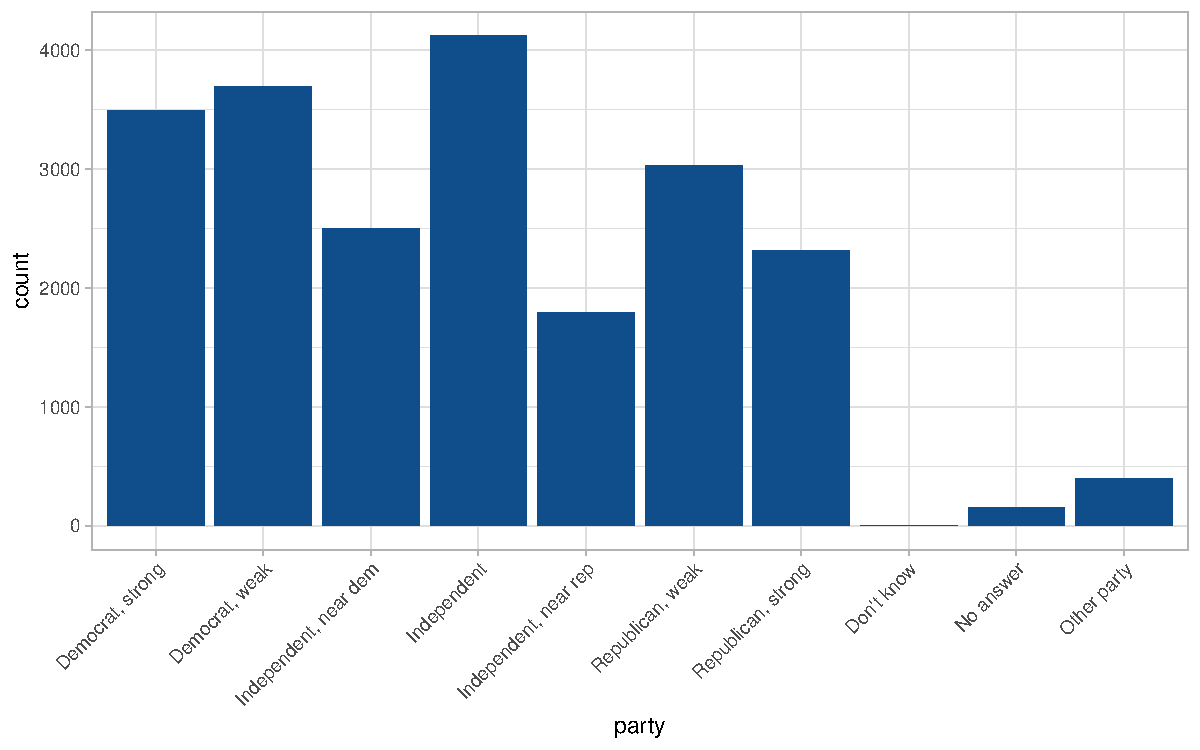
\includegraphics{cleaning_tutorial_files/figure-latex/unnamed-chunk-29-1}

In conclusion we use

\begin{itemize}
\tightlist
\item
  \texttt{fct\_recode} for recoding values of a categorical variable,
  and
\item
  \texttt{fct\_relevel} for manually reordering values of a categorical
  variable.
\end{itemize}

Later on, we will seen more specific functions for recoding and
reordering categorical variables when transforming data. Make sure you
don't lose the overview! First, we look at cleaning continuous data.

\section{Cleaning continuous data}\label{cleaning-continuous-data}

For continuous data, the range of possible values is infinite, and it is
therefore more difficult to find \emph{wrong} values. Without
information on the context of the data, finding wrong continuous entries
is extremely difficult.

\subsection{Errors}\label{errors}

In the \texttt{survey} data.frame, there are three continuous variables:
year, age and (daily) tv\_hours. For each of these variables, we have a
certain idea about the possible range of values. The age will probably
by somewhere between 20 and 100 (knowing that the dataset contains
information on adults). The number of tv hours should be between 0 and
24, as there are 24 hours in a day. Also for year we more or less know
what to expect. Let's have a look at each. \footnote{When inspecting
  categorical data, we can do a quick count. While this might work for
  some continuous variables, such as year, it is not suited for most
  continuous variables, as they are often unique for each observation.
  Instead, we look at the summary of the variables.}

\begin{Shaded}
\begin{Highlighting}[]
\KeywordTok{summary}\NormalTok{(survey}\OperatorTok{$}\NormalTok{year)}
\end{Highlighting}
\end{Shaded}

\begin{verbatim}
##    Min. 1st Qu.  Median    Mean 3rd Qu. 
##    2000    2002    2006    2007    2010 
##    Max. 
##    2014
\end{verbatim}

For year, everything seems allright. We converted it already to an
integer variable before, so we don't have to check for erroneous decimal
years. Furthermore, the minimum and maximum seems quite alright. When
year contains errors, we most likely observe it at thise extremes: 2102
instead of 2012, 1099 instead of 1999, or 9999 indicating that it is
actually missing.

Let's look at age then.

\begin{Shaded}
\begin{Highlighting}[]
\KeywordTok{summary}\NormalTok{(survey}\OperatorTok{$}\NormalTok{age)}
\end{Highlighting}
\end{Shaded}

\begin{verbatim}
##    Min. 1st Qu.  Median    Mean 3rd Qu. 
##   18.00   33.00   46.00   47.18   59.00 
##    Max.    NA's 
##   89.00      76
\end{verbatim}

On first sight, there does not seem to be problems with age. There are
76 missing values, but the values present are situated between 18 and 89
years, which again is a logical range. Also age was converted without
problems to an integer variable before, so all values are integer
numbers.

If we look at tv hours, we see something peculiar.

\begin{Shaded}
\begin{Highlighting}[]
\KeywordTok{summary}\NormalTok{(survey}\OperatorTok{$}\NormalTok{tv_hours)}
\end{Highlighting}
\end{Shaded}

\begin{verbatim}
##    Min. 1st Qu.  Median    Mean 3rd Qu. 
##   0.000   1.000   2.000   3.004   4.000 
##    Max.    NA's 
##  84.000   10146
\end{verbatim}

We see there are 10146 missing values, which is high but not necessarily
wrong (unless we accidently removed some values, which we didn't). There
are no negative values, as the minimum number of hours someone watched
tv is zero. However, on the other side, we see that the number of tv
hours goes up to 84 hours a day - this is clearly wrong. We all have
just 24 hours in a day.

We can further look at the records for which the tv hours are more than
24.

\begin{Shaded}
\begin{Highlighting}[]
\NormalTok{survey }\OperatorTok\StringTok{ }\KeywordTok{filter}\NormalTok{(tv_hours }\OperatorTok{>}\StringTok{ }\DecValTok{24}\NormalTok{)}
\end{Highlighting}
\end{Shaded}

\begin{verbatim}
## # A tibble: 5 x 9
##    year marital   age race  reported_income
##   <dbl> <fct>   <dbl> <fct> <ord>          
## 1  2000 Married    84 White Not applicable 
## 2  2000 Widowed    68 White Not applicable 
## 3  2010 Married    69 White Not applicable 
## 4  2010 Divorc~    57 White Not applicable 
## 5  2014 Separa~    30 White Not applicable 
## # ... with 4 more variables: party <fct>,
## #   religion <fct>, denomination <fct>,
## #   tv_hours <dbl>
\end{verbatim}

There seem to be 5 observations for which the number of tv hours is
clearly wrong, and we need to correct them. However, we don't have a
clue how to correct them in our case. The only thing we can do, is to
deleted these values, and make them missing. \footnote{Errors such as
  these can often be avoided by proper data collection I.e., if you
  create a survey or a data form online, make sure that all fields are
  reasonably checked: age cannot be negative, a zip code consists of 4
  numbers, and one does not have more than 24 hours in a day. While
  there are still things which can go wrong later, at least the data
  cannot be wrongly inputted by respondents. In real-life, many data
  collection happens without much thought, unfortunately.} Observe, we
do not delete the entire observations, just the tvhours variable for
these observations. The other variables can still be used for these 5
rows.

We can do this by using the \texttt{ifelse} function. This function is a
very generic function which returns a value dependent on a logical
test.\footnote{Maybe you are familiar with the \texttt{IF} function in
  Excel? It's use is exactly the same.} The function can be used as
follows.

\begin{Shaded}
\begin{Highlighting}[]
\KeywordTok{if_else}\NormalTok{( }\OperatorTok{<}\NormalTok{condition}\OperatorTok{>}\NormalTok{, }\OperatorTok{<}\NormalTok{value_a}\OperatorTok{>}\NormalTok{, }\OperatorTok{<}\NormalTok{value_b}\OperatorTok{>}\StringTok{ }\NormalTok{)}
\end{Highlighting}
\end{Shaded}

Suppose we have a vector \texttt{score} containing student scores. We
can use the \texttt{ifelse} function to create a vector \texttt{grade}
with values \texttt{FAILED} and \texttt{PASSED}.

\begin{Shaded}
\begin{Highlighting}[]
\NormalTok{grade <-}\StringTok{ }\KeywordTok{ifelse}\NormalTok{(score }\OperatorTok{>=}\StringTok{ }\DecValTok{10}\NormalTok{, }\StringTok{"PASSED"}\NormalTok{, }\StringTok{"FAILED"}\NormalTok{)}
\end{Highlighting}
\end{Shaded}

Now, let's use the function to update the tv hours variable.

\begin{Shaded}
\begin{Highlighting}[]
\NormalTok{survey <-}\StringTok{ }\NormalTok{survey }\OperatorTok\StringTok{ }\KeywordTok{mutate}\NormalTok{(}\DataTypeTok{tv_hours =} \KeywordTok{ifelse}\NormalTok{(tv_hours }\OperatorTok{>}\StringTok{ }
\StringTok{    }\DecValTok{24}\NormalTok{, }\OtherTok{NA}\NormalTok{, tv_hours))}
\end{Highlighting}
\end{Shaded}

So, what happens? The tv\_hours variable is updated using
\texttt{mutate}. If it is larger than 24, the new value will be
\texttt{NA}, i.e.~not available. Otherwise, the new value will just be
the old value of tv\_hours. After the column is updated, the new
data.frame is again stored as \texttt{survey}.

Checking for errors, both categorical and continuous, can be a
\emph{street without ending}. Usually, you do the best you can by using
the tricks discussed above for each variable. If this seems like a lot
of work, remember that 70\% of a typical data project goes to cleaning
and transforming data, and only 30\% to actual analysis and
interpretation.

And even then, despite all your time and efforts, in can happen that
your discover data errors in the analysis phase. Not surprisingly, as
you will really look at the data in detail at that point. When this
happens, you go back to your cleaning and transformation scripts and
modify them where needed. As such, it is important that you store the
original data as well as all the changes you performed. Even more
important is to make sure that all your analysis are stored as a script
of RMarkdown, so that they can quickly be rerun after correcting the
error. This is called \emph{reproducible research} and will save you a
lot of time and mistakes. Have a look at
\href{https://www.youtube.com/watch?v=s3JldKoA0zw}{this video} for an
illustration of reproducible work-flows.

\subsection{Outliers}\label{outliers}

It also happens that some continuous values are not necessarily wrong,
but \emph{exceptionally} high or low. These exceptions we don't call
error, but instead we call outliers -- a data point that is distant from
other observations. For example, consider tv hours. Before we removed
values greater than 24 hours, because there are logically errors. Let's
have a look at the remaining values.

\begin{Shaded}
\begin{Highlighting}[]
\NormalTok{survey }\OperatorTok\StringTok{ }\KeywordTok{ggplot}\NormalTok{(}\KeywordTok{aes}\NormalTok{(tv_hours)) }\OperatorTok{+}\StringTok{ }\KeywordTok{geom_histogram}\NormalTok{(}\DataTypeTok{binwidth =} \DecValTok{1}\NormalTok{, }
    \DataTypeTok{color =} \StringTok{"white"}\NormalTok{, }\DataTypeTok{fill =} \StringTok{"dodgerblue4"}\NormalTok{) }\OperatorTok{+}\StringTok{ }\KeywordTok{theme_light}\NormalTok{()}
\end{Highlighting}
\end{Shaded}

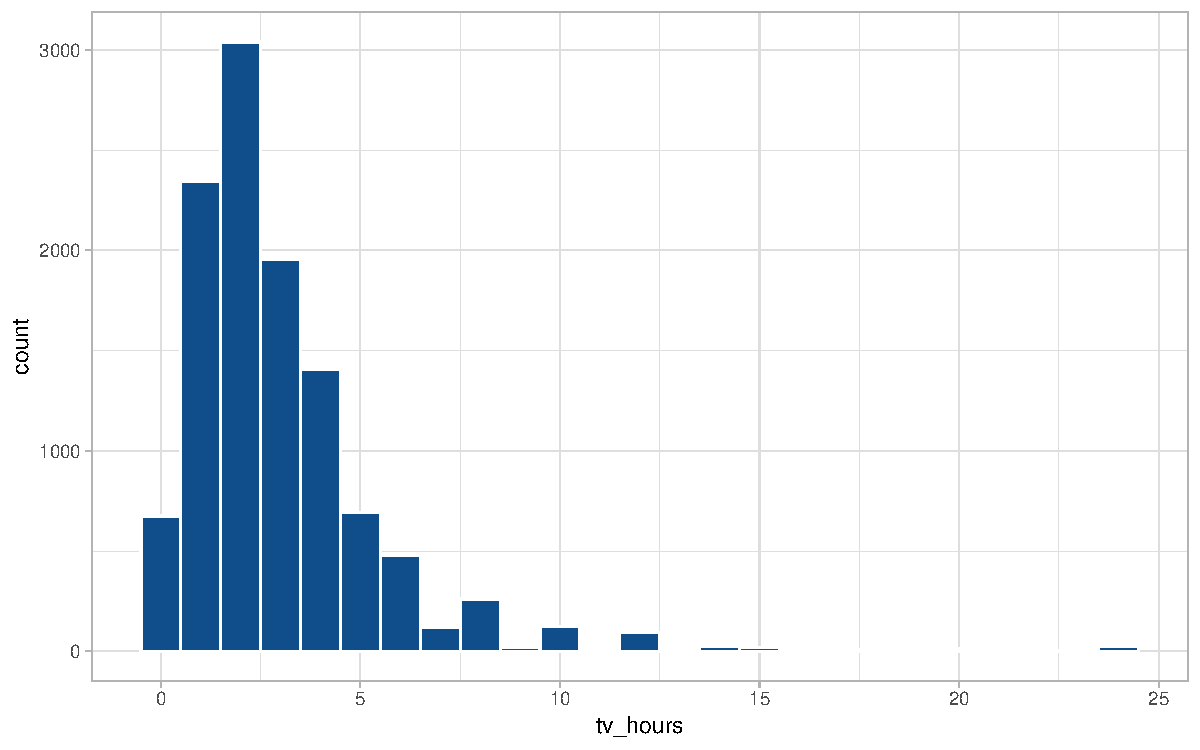
\includegraphics{cleaning_tutorial_files/figure-latex/unnamed-chunk-37-1}

It seems that while most people watch television between 0 and 5 hour a
day, there are some exceptionally high values. It's not clear whether
they are mistakes like the onces we removed before, or just abnormal
tv-addicts. Let's have a look at the 25 highest values, and compare them
with some related attributes, such as age, income and marital status
(comparing them with religion or party might be regarded as politically
incorrect, so let's steer clear from that danger zone).\footnote{Remember
  that we use pander to improve the layout of our tables, and you
  shouldn't pay attention to that.}

\begin{Shaded}
\begin{Highlighting}[]
\NormalTok{survey }\OperatorTok\StringTok{ }\KeywordTok{arrange}\NormalTok{(}\OperatorTok{-}\NormalTok{tv_hours) }\OperatorTok\StringTok{ }\KeywordTok{slice}\NormalTok{(}\DecValTok{1}\OperatorTok{:}\DecValTok{25}\NormalTok{) }\OperatorTok\StringTok{ }
\StringTok{    }\KeywordTok{select}\NormalTok{(tv_hours, marital, age, reported_income) }\OperatorTok\StringTok{ }
\StringTok{    }\KeywordTok{pander}\NormalTok{()}
\end{Highlighting}
\end{Shaded}

\begin{longtable}[]{@{}cccc@{}}
\toprule
\begin{minipage}[b]{0.14\columnwidth}\centering\strut
tv\_hours\strut
\end{minipage} & \begin{minipage}[b]{0.20\columnwidth}\centering\strut
marital\strut
\end{minipage} & \begin{minipage}[b]{0.07\columnwidth}\centering\strut
age\strut
\end{minipage} & \begin{minipage}[b]{0.21\columnwidth}\centering\strut
reported\_income\strut
\end{minipage}\tabularnewline
\midrule
\endhead
\begin{minipage}[t]{0.14\columnwidth}\centering\strut
24\strut
\end{minipage} & \begin{minipage}[t]{0.20\columnwidth}\centering\strut
Never married\strut
\end{minipage} & \begin{minipage}[t]{0.07\columnwidth}\centering\strut
30\strut
\end{minipage} & \begin{minipage}[t]{0.21\columnwidth}\centering\strut
Not applicable\strut
\end{minipage}\tabularnewline
\begin{minipage}[t]{0.14\columnwidth}\centering\strut
24\strut
\end{minipage} & \begin{minipage}[t]{0.20\columnwidth}\centering\strut
Separated\strut
\end{minipage} & \begin{minipage}[t]{0.07\columnwidth}\centering\strut
45\strut
\end{minipage} & \begin{minipage}[t]{0.21\columnwidth}\centering\strut
Not applicable\strut
\end{minipage}\tabularnewline
\begin{minipage}[t]{0.14\columnwidth}\centering\strut
24\strut
\end{minipage} & \begin{minipage}[t]{0.20\columnwidth}\centering\strut
Never married\strut
\end{minipage} & \begin{minipage}[t]{0.07\columnwidth}\centering\strut
33\strut
\end{minipage} & \begin{minipage}[t]{0.21\columnwidth}\centering\strut
\$6000 to 6999\strut
\end{minipage}\tabularnewline
\begin{minipage}[t]{0.14\columnwidth}\centering\strut
24\strut
\end{minipage} & \begin{minipage}[t]{0.20\columnwidth}\centering\strut
Divorced\strut
\end{minipage} & \begin{minipage}[t]{0.07\columnwidth}\centering\strut
53\strut
\end{minipage} & \begin{minipage}[t]{0.21\columnwidth}\centering\strut
Not applicable\strut
\end{minipage}\tabularnewline
\begin{minipage}[t]{0.14\columnwidth}\centering\strut
24\strut
\end{minipage} & \begin{minipage}[t]{0.20\columnwidth}\centering\strut
Divorced\strut
\end{minipage} & \begin{minipage}[t]{0.07\columnwidth}\centering\strut
50\strut
\end{minipage} & \begin{minipage}[t]{0.21\columnwidth}\centering\strut
No answer\strut
\end{minipage}\tabularnewline
\begin{minipage}[t]{0.14\columnwidth}\centering\strut
24\strut
\end{minipage} & \begin{minipage}[t]{0.20\columnwidth}\centering\strut
Never married\strut
\end{minipage} & \begin{minipage}[t]{0.07\columnwidth}\centering\strut
44\strut
\end{minipage} & \begin{minipage}[t]{0.21\columnwidth}\centering\strut
Not applicable\strut
\end{minipage}\tabularnewline
\begin{minipage}[t]{0.14\columnwidth}\centering\strut
24\strut
\end{minipage} & \begin{minipage}[t]{0.20\columnwidth}\centering\strut
Never married\strut
\end{minipage} & \begin{minipage}[t]{0.07\columnwidth}\centering\strut
21\strut
\end{minipage} & \begin{minipage}[t]{0.21\columnwidth}\centering\strut
Don't know\strut
\end{minipage}\tabularnewline
\begin{minipage}[t]{0.14\columnwidth}\centering\strut
24\strut
\end{minipage} & \begin{minipage}[t]{0.20\columnwidth}\centering\strut
Widowed\strut
\end{minipage} & \begin{minipage}[t]{0.07\columnwidth}\centering\strut
71\strut
\end{minipage} & \begin{minipage}[t]{0.21\columnwidth}\centering\strut
Not applicable\strut
\end{minipage}\tabularnewline
\begin{minipage}[t]{0.14\columnwidth}\centering\strut
24\strut
\end{minipage} & \begin{minipage}[t]{0.20\columnwidth}\centering\strut
Widowed\strut
\end{minipage} & \begin{minipage}[t]{0.07\columnwidth}\centering\strut
62\strut
\end{minipage} & \begin{minipage}[t]{0.21\columnwidth}\centering\strut
Not applicable\strut
\end{minipage}\tabularnewline
\begin{minipage}[t]{0.14\columnwidth}\centering\strut
24\strut
\end{minipage} & \begin{minipage}[t]{0.20\columnwidth}\centering\strut
Widowed\strut
\end{minipage} & \begin{minipage}[t]{0.07\columnwidth}\centering\strut
52\strut
\end{minipage} & \begin{minipage}[t]{0.21\columnwidth}\centering\strut
Refused\strut
\end{minipage}\tabularnewline
\begin{minipage}[t]{0.14\columnwidth}\centering\strut
24\strut
\end{minipage} & \begin{minipage}[t]{0.20\columnwidth}\centering\strut
Never married\strut
\end{minipage} & \begin{minipage}[t]{0.07\columnwidth}\centering\strut
56\strut
\end{minipage} & \begin{minipage}[t]{0.21\columnwidth}\centering\strut
Not applicable\strut
\end{minipage}\tabularnewline
\begin{minipage}[t]{0.14\columnwidth}\centering\strut
24\strut
\end{minipage} & \begin{minipage}[t]{0.20\columnwidth}\centering\strut
Divorced\strut
\end{minipage} & \begin{minipage}[t]{0.07\columnwidth}\centering\strut
51\strut
\end{minipage} & \begin{minipage}[t]{0.21\columnwidth}\centering\strut
Not applicable\strut
\end{minipage}\tabularnewline
\begin{minipage}[t]{0.14\columnwidth}\centering\strut
24\strut
\end{minipage} & \begin{minipage}[t]{0.20\columnwidth}\centering\strut
Divorced\strut
\end{minipage} & \begin{minipage}[t]{0.07\columnwidth}\centering\strut
75\strut
\end{minipage} & \begin{minipage}[t]{0.21\columnwidth}\centering\strut
Not applicable\strut
\end{minipage}\tabularnewline
\begin{minipage}[t]{0.14\columnwidth}\centering\strut
24\strut
\end{minipage} & \begin{minipage}[t]{0.20\columnwidth}\centering\strut
Separated\strut
\end{minipage} & \begin{minipage}[t]{0.07\columnwidth}\centering\strut
49\strut
\end{minipage} & \begin{minipage}[t]{0.21\columnwidth}\centering\strut
\$8000 to 9999\strut
\end{minipage}\tabularnewline
\begin{minipage}[t]{0.14\columnwidth}\centering\strut
24\strut
\end{minipage} & \begin{minipage}[t]{0.20\columnwidth}\centering\strut
Divorced\strut
\end{minipage} & \begin{minipage}[t]{0.07\columnwidth}\centering\strut
65\strut
\end{minipage} & \begin{minipage}[t]{0.21\columnwidth}\centering\strut
Not applicable\strut
\end{minipage}\tabularnewline
\begin{minipage}[t]{0.14\columnwidth}\centering\strut
24\strut
\end{minipage} & \begin{minipage}[t]{0.20\columnwidth}\centering\strut
Never married\strut
\end{minipage} & \begin{minipage}[t]{0.07\columnwidth}\centering\strut
27\strut
\end{minipage} & \begin{minipage}[t]{0.21\columnwidth}\centering\strut
Not applicable\strut
\end{minipage}\tabularnewline
\begin{minipage}[t]{0.14\columnwidth}\centering\strut
24\strut
\end{minipage} & \begin{minipage}[t]{0.20\columnwidth}\centering\strut
Married\strut
\end{minipage} & \begin{minipage}[t]{0.07\columnwidth}\centering\strut
71\strut
\end{minipage} & \begin{minipage}[t]{0.21\columnwidth}\centering\strut
Not applicable\strut
\end{minipage}\tabularnewline
\begin{minipage}[t]{0.14\columnwidth}\centering\strut
24\strut
\end{minipage} & \begin{minipage}[t]{0.20\columnwidth}\centering\strut
Never married\strut
\end{minipage} & \begin{minipage}[t]{0.07\columnwidth}\centering\strut
27\strut
\end{minipage} & \begin{minipage}[t]{0.21\columnwidth}\centering\strut
\$8000 to 9999\strut
\end{minipage}\tabularnewline
\begin{minipage}[t]{0.14\columnwidth}\centering\strut
24\strut
\end{minipage} & \begin{minipage}[t]{0.20\columnwidth}\centering\strut
Separated\strut
\end{minipage} & \begin{minipage}[t]{0.07\columnwidth}\centering\strut
63\strut
\end{minipage} & \begin{minipage}[t]{0.21\columnwidth}\centering\strut
Not applicable\strut
\end{minipage}\tabularnewline
\begin{minipage}[t]{0.14\columnwidth}\centering\strut
24\strut
\end{minipage} & \begin{minipage}[t]{0.20\columnwidth}\centering\strut
Divorced\strut
\end{minipage} & \begin{minipage}[t]{0.07\columnwidth}\centering\strut
31\strut
\end{minipage} & \begin{minipage}[t]{0.21\columnwidth}\centering\strut
\$5000 to 5999\strut
\end{minipage}\tabularnewline
\begin{minipage}[t]{0.14\columnwidth}\centering\strut
24\strut
\end{minipage} & \begin{minipage}[t]{0.20\columnwidth}\centering\strut
Separated\strut
\end{minipage} & \begin{minipage}[t]{0.07\columnwidth}\centering\strut
37\strut
\end{minipage} & \begin{minipage}[t]{0.21\columnwidth}\centering\strut
Not applicable\strut
\end{minipage}\tabularnewline
\begin{minipage}[t]{0.14\columnwidth}\centering\strut
24\strut
\end{minipage} & \begin{minipage}[t]{0.20\columnwidth}\centering\strut
Married\strut
\end{minipage} & \begin{minipage}[t]{0.07\columnwidth}\centering\strut
46\strut
\end{minipage} & \begin{minipage}[t]{0.21\columnwidth}\centering\strut
Not applicable\strut
\end{minipage}\tabularnewline
\begin{minipage}[t]{0.14\columnwidth}\centering\strut
23\strut
\end{minipage} & \begin{minipage}[t]{0.20\columnwidth}\centering\strut
Never married\strut
\end{minipage} & \begin{minipage}[t]{0.07\columnwidth}\centering\strut
32\strut
\end{minipage} & \begin{minipage}[t]{0.21\columnwidth}\centering\strut
Not applicable\strut
\end{minipage}\tabularnewline
\begin{minipage}[t]{0.14\columnwidth}\centering\strut
22\strut
\end{minipage} & \begin{minipage}[t]{0.20\columnwidth}\centering\strut
Divorced\strut
\end{minipage} & \begin{minipage}[t]{0.07\columnwidth}\centering\strut
69\strut
\end{minipage} & \begin{minipage}[t]{0.21\columnwidth}\centering\strut
Not applicable\strut
\end{minipage}\tabularnewline
\begin{minipage}[t]{0.14\columnwidth}\centering\strut
22\strut
\end{minipage} & \begin{minipage}[t]{0.20\columnwidth}\centering\strut
Married\strut
\end{minipage} & \begin{minipage}[t]{0.07\columnwidth}\centering\strut
63\strut
\end{minipage} & \begin{minipage}[t]{0.21\columnwidth}\centering\strut
Not applicable\strut
\end{minipage}\tabularnewline
\bottomrule
\end{longtable}

It seems that many of the respondents watch the maximum number of 24
hours tv each day, which is surprising. We can use the other variables
to get a better idea about these observations. We see that many of them
are single (never married, divorced or separated). The age seems to be
relatively high, but not very remarkable (average age for the dataset
was about 47). Finally, many did not report their income.

This information can be interpreted in multiple ways:

\begin{itemize}
\tightlist
\item
  These are single, lazy people with an income who watch tv all day
\item
  These are people who weren't very honest when filling out their
  information (also not reporting any income).
\end{itemize}

Deciding whether something is wrong or exceptional is not trivial and
requires certain domain knowledge and assumptions. In this case, the
logical assumption is that these numbers are incorrect (even lazy,
tv-binging people need to sleep now and then). The more difficult
question is at what point something becomes incorrect. 20 hours? 16? For
continuous variables it can help to look at a boxplot and see until
where the whiskers go. However, this is no exact science, especially
when variables are not distributed symmetrically.

\begin{Shaded}
\begin{Highlighting}[]
\NormalTok{survey }\OperatorTok\StringTok{ }\KeywordTok{ggplot}\NormalTok{(}\KeywordTok{aes}\NormalTok{(}\StringTok{""}\NormalTok{, tv_hours)) }\OperatorTok{+}\StringTok{ }\KeywordTok{geom_boxplot}\NormalTok{()}
\end{Highlighting}
\end{Shaded}

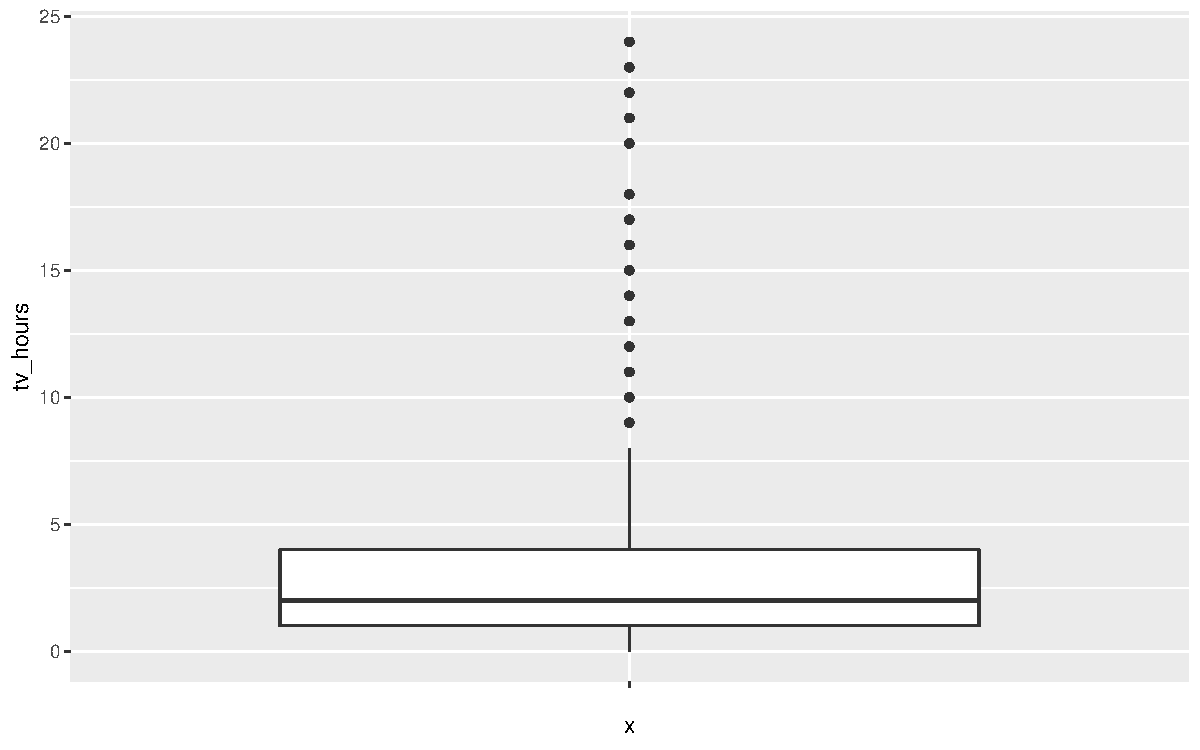
\includegraphics{cleaning_tutorial_files/figure-latex/unnamed-chunk-39-1}

For the current case, we can say the people who watch more than 8 hours
tv either filled in an incorrect number, or are exceptional tv-watchers.
As such, we remove all values higher than 8.

\begin{Shaded}
\begin{Highlighting}[]
\NormalTok{survey <-}\StringTok{ }\NormalTok{survey }\OperatorTok\StringTok{ }\KeywordTok{mutate}\NormalTok{(}\DataTypeTok{tv_hours =} \KeywordTok{ifelse}\NormalTok{(tv_hours }\OperatorTok{>}\StringTok{ }
\StringTok{    }\DecValTok{8}\NormalTok{, }\OtherTok{NA}\NormalTok{, tv_hours))}
\end{Highlighting}
\end{Shaded}

\section{Data inconsistencies}\label{data-inconsistencies}

Another approach to check for errors is to look at more than one
variable at the same time, and check for obvious inconsistencies. This
can be though of as ``rules'' which are violated. In the current
dataset, we could check that all married people should be at least 18
years old. Since all observations concern people which are at least 18
years old, we know that this rule is not violated.

In other cases, example rules can be:

\begin{itemize}
\tightlist
\item
  the departure of a flight should take place before it can arrive.
  (Taking into account different time zones, obviously.)
\item
  someone whose job status is ``unemployed'' cannot have a reported
  income (unless unemployment benefits are taken into account).
\item
  etc.
\end{itemize}

Often, you will not have time to check all posible rules you can think
of. Furthermore, some rules will be based on certain assumptions which
you need to check. For example, the
\href{https://en.wikipedia.org/wiki/Marriageable_age}{age at which one
can marry} depends on the country, and thus be lower or higher than 18.

\section{Missing values}\label{missing-values}

In a real-life setting, data typically comes with missing values. The
values might be missing from the offset, or they might be missing
because we removed them as outliers or wrong values. In subsequent
paragraphs we will see how to analyse missing values -- e.g.~are they
missing at random or not? -- and how to handle them during your
analysis. We are obliged to say that there are also techniques which can
be used to \emph{guess} missing values based on the values for other
attributes and other observations with similar values. This is called
missing value \emph{imputation} and as a separate field on itself. Due
to the complexities involved, we will not talk about it here, but the
interested reader is refered to
\href{https://datascienceplus.com/imputing-missing-data-with-r-mice-package/}{this
manual of the mice-package}.

\subsection{Analyzing missing data}\label{analyzing-missing-data}

There are three different ways in which missing data can occur (see
theory).

\begin{itemize}
\tightlist
\item
  Missing Completely at Random (MCAR)
\item
  Missing at Random (MAR)
\item
  Not Missing at Random (NMAR)
\end{itemize}

Below, we illustrate some techniques to analyse the missing values in
your data. The most obvious way to check whether your data contains
missing values is by looking at the summary.

\begin{Shaded}
\begin{Highlighting}[]
\KeywordTok{summary}\NormalTok{(survey)}
\end{Highlighting}
\end{Shaded}

\begin{verbatim}
##       year               marital     
##  Min.   :2000   Divorced     : 3383  
##  1st Qu.:2002   Married      :10117  
##  Median :2006   Never married: 5416  
##  Mean   :2007   No answer    :   17  
##  3rd Qu.:2010   Separated    :  743  
##  Max.   :2014   Widowed      : 1807  
##                                      
##       age           race      
##  Min.   :18.00   Black: 3129  
##  1st Qu.:33.00   Other: 1959  
##  Median :46.00   White:16395  
##  Mean   :47.18                
##  3rd Qu.:59.00                
##  Max.   :89.00                
##  NA's   :76                   
##        reported_income
##  $25000 or more:7363  
##  Not applicable:7043  
##  $20000 - 24999:1283  
##  $10000 - 14999:1168  
##  $15000 - 19999:1048  
##  Refused       : 975  
##  (Other)       :2603  
##                    party     
##  Independent          :4119  
##  Democrat, weak       :3690  
##  Democrat, strong     :3490  
##  Republican, weak     :3032  
##  Independent, near dem:2499  
##  Republican, strong   :2314  
##  (Other)              :2339  
##        religion               denomination  
##  Protestant:10846   Not applicable  :10072  
##  Catholic  : 5124   Other           : 2534  
##  None      : 3523   No denomination : 1683  
##  Christian :  689   Southern baptist: 1536  
##  Jewish    :  388   Baptist-dk which: 1457  
##  Other     :  224   United methodist: 1067  
##  (Other)   :  689   (Other)         : 3134  
##     tv_hours    
##  Min.   :0.000  
##  1st Qu.:1.000  
##  Median :2.000  
##  Mean   :2.659  
##  3rd Qu.:4.000  
##  Max.   :8.000  
##  NA's   :10509
\end{verbatim}

This tells us for which variables there are missing data, and how many.
However, it does not tell us anything about the relationships between
missing values. In order to look at \emph{patterns} of missing data, we
can use the \texttt{md.pattern} function (missing data patterns) from
the package \texttt{mice}.

\begin{Shaded}
\begin{Highlighting}[]
\KeywordTok{md.pattern}\NormalTok{(survey)}
\end{Highlighting}
\end{Shaded}

\begin{verbatim}
##       year marital race reported_income
## 10936    1       1    1               1
##    38    1       1    1               1
## 10471    1       1    1               1
##    38    1       1    1               1
##          0       0    0               0
##       party religion denomination age
## 10936     1        1            1   1
##    38     1        1            1   0
## 10471     1        1            1   1
##    38     1        1            1   0
##           0        0            0  76
##       tv_hours      
## 10936        1     0
##    38        1     1
## 10471        0     1
##    38        0     2
##          10509 10585
\end{verbatim}

The output of \texttt{md.pattern} is a bit cryptic, but let's have a
closer look. Each column refers to one of the variables, as is
indicated. Each row is a \emph{pattern} consisting of 1s (data is not
missing) and 0s (data is missing). The first row, where all variables
have a 1, is a pattern where non of the variables is missing. This is
also denoted by the zero in the last column. In the second rows, age is
indicated with a zero, meaning that for this pattern, the variable age
is missing. The last column thus indicates 1 missing value. The last
pattern (the penultimate row) is one with 2 missing values as indicated
in the last column. In particular, age and tv hours are missing.

The number is the first (unnamed) column indicate how many observations
of each pattern there are. As such, the first pattern has the most
observations -- 10936 persons without missing data. The last pattern (tv
hours and age missing) occurs 38 times. The final row equals the number
of missing values for each variable (the same information summary gave
us). Finally, the number in the lower-right corner is the total number
of missing values.

The output of md.patterns can show us whether the occurence of missing
values are related. For example, if age is missing, then tv hourse is
also missing. The latter is not the case, as there are as many
observaties where age is missing and tv hours not, as there are
observations were age is missing and tv hours also.

Next to \texttt{md.pattern} we can also check whether the occurence of
missing values is related to the value for other variables. As such, we
can ask ourselves whether people from certain religions or political
affiliations are more or less likely to report there age our the number
of hours they watch tv. These patterns can be checked using
ggplot/dplyr, by creating a new variable that indicates whether an
observation has a missing value.

Let's consider age. We add a variable to indicate that age is or is not
missing. Note that to check this, we need a special function. We cannot
use age == NA to see if age is missing. In the latter condition, we are
comparing age with NA, i.e.~we are comparing age with something we don't
have. We can never know whether age is equal to something we don't have,
so the result of that is always NA, regardless of the value of age. As
an example, consider the variables a and b, of which a is missing and b
is not.

\begin{Shaded}
\begin{Highlighting}[]
\NormalTok{a <-}\StringTok{ }\OtherTok{NA}
\NormalTok{b <-}\StringTok{ }\DecValTok{1}

\NormalTok{a }\OperatorTok{==}\StringTok{ }\OtherTok{NA}
\end{Highlighting}
\end{Shaded}

\begin{verbatim}
## [1] NA
\end{verbatim}

\begin{Shaded}
\begin{Highlighting}[]
\NormalTok{b }\OperatorTok{==}\StringTok{ }\OtherTok{NA}
\end{Highlighting}
\end{Shaded}

\begin{verbatim}
## [1] NA
\end{verbatim}

So, how do we check if something is NA? We use the special function
\texttt{is.na} for that.

\begin{Shaded}
\begin{Highlighting}[]
\KeywordTok{is.na}\NormalTok{(a)}
\end{Highlighting}
\end{Shaded}

\begin{verbatim}
## [1] TRUE
\end{verbatim}

\begin{Shaded}
\begin{Highlighting}[]
\KeywordTok{is.na}\NormalTok{(b)}
\end{Highlighting}
\end{Shaded}

\begin{verbatim}
## [1] FALSE
\end{verbatim}

Thus, for the survey data:

\begin{Shaded}
\begin{Highlighting}[]
\NormalTok{survey_md <-}\StringTok{ }\NormalTok{survey }\OperatorTok\StringTok{ }\KeywordTok{mutate}\NormalTok{(}\DataTypeTok{age_missing =} \KeywordTok{is.na}\NormalTok{(age), }
    \DataTypeTok{tv_missing =} \KeywordTok{is.na}\NormalTok{(tv_hours))}
\end{Highlighting}
\end{Shaded}

Note that we store the data.frame with the additional variables under
another name, since we will not need these variables in the eventual
analysis stage, just for looking at the missing data for the moment.

When we compare the missing/not missing variable with a categorical
variable, we have in fact 2 categorical variables. Thus, we can use a
graph or table which is appropriate for comparing categorical variables.
As we all (should) know by now, we can use a bar chart.

\begin{Shaded}
\begin{Highlighting}[]
\NormalTok{survey_md }\OperatorTok\StringTok{ }\KeywordTok{ggplot}\NormalTok{(}\KeywordTok{aes}\NormalTok{(reported_income, }\DataTypeTok{fill =}\NormalTok{ age_missing)) }\OperatorTok{+}\StringTok{ }
\StringTok{    }\KeywordTok{geom_bar}\NormalTok{(}\DataTypeTok{position =} \StringTok{"fill"}\NormalTok{) }\OperatorTok{+}\StringTok{ }\KeywordTok{coord_flip}\NormalTok{()}
\end{Highlighting}
\end{Shaded}

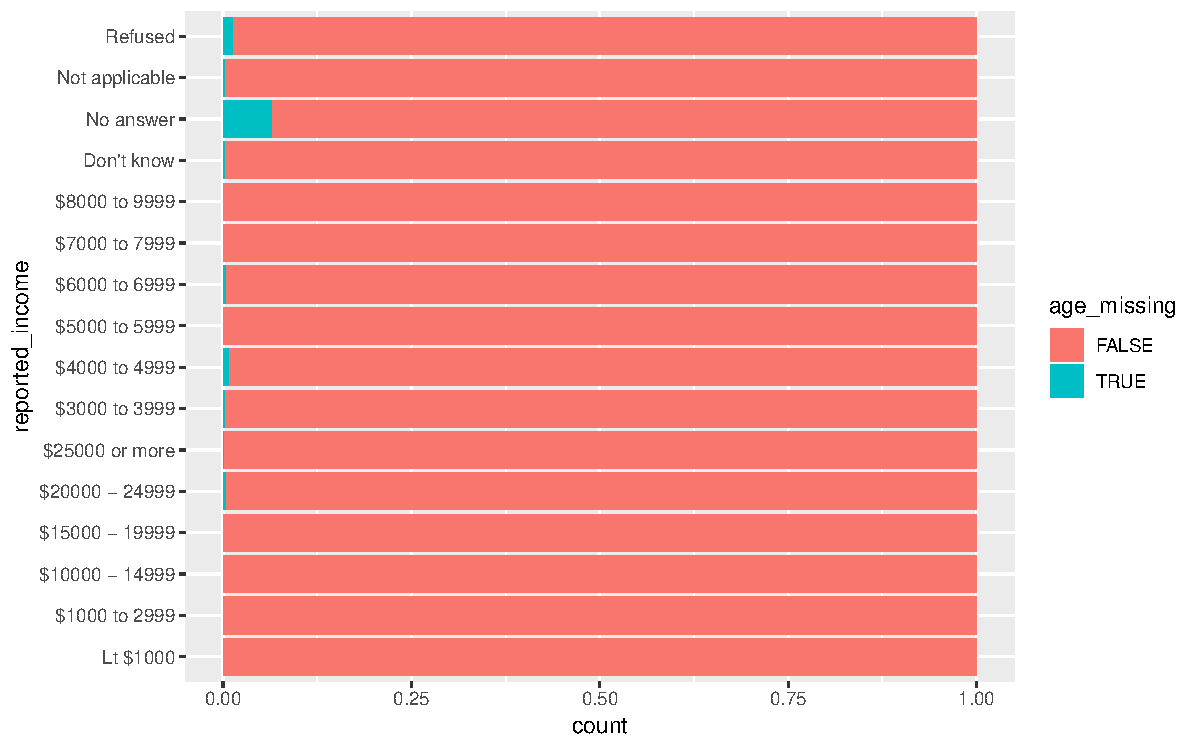
\includegraphics{cleaning_tutorial_files/figure-latex/unnamed-chunk-46-1}

The bar chart shows that people who didn't report their income, were
more likely to not report their age also. \footnote{One could argue that
  we also coded the ``No answer'' value for reported income as NA.
  However, it this case, it was decided not to, in order to retain a
  clear distinction between the special categories (Refused, Not
  applicable, No answer and Don't know).}.

We can do the same for tv-hours. We then see that the percentage of
missing values varies -- being somewhat higher or lower for certain
incomes -- but no clear patterns exist.

\begin{Shaded}
\begin{Highlighting}[]
\NormalTok{survey_md }\OperatorTok\StringTok{ }\KeywordTok{ggplot}\NormalTok{(}\KeywordTok{aes}\NormalTok{(reported_income, }\DataTypeTok{fill =}\NormalTok{ tv_missing)) }\OperatorTok{+}\StringTok{ }
\StringTok{    }\KeywordTok{geom_bar}\NormalTok{(}\DataTypeTok{position =} \StringTok{"fill"}\NormalTok{) }\OperatorTok{+}\StringTok{ }\KeywordTok{coord_flip}\NormalTok{()}
\end{Highlighting}
\end{Shaded}

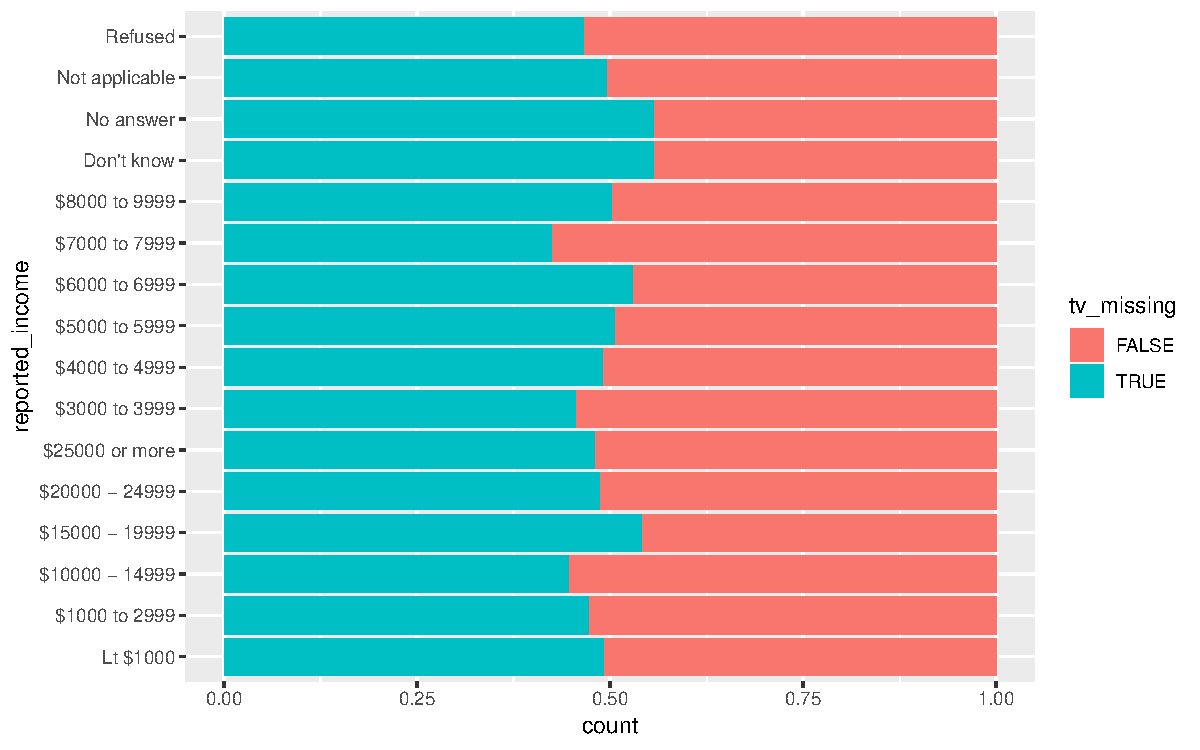
\includegraphics{cleaning_tutorial_files/figure-latex/unnamed-chunk-47-1}

Of course, the occurence of missing values can be compared with more
than one variable, not just income. Below we show the comparison of
tv-hours missing with political affiliation. Here we can clearly see
that there is one answer for political party which was only used for
observations which did not include the tv hours.

\begin{Shaded}
\begin{Highlighting}[]
\NormalTok{survey_md }\OperatorTok\StringTok{ }\KeywordTok{ggplot}\NormalTok{(}\KeywordTok{aes}\NormalTok{(party, }\DataTypeTok{fill =}\NormalTok{ tv_missing)) }\OperatorTok{+}\StringTok{ }
\StringTok{    }\KeywordTok{geom_bar}\NormalTok{(}\DataTypeTok{position =} \StringTok{"fill"}\NormalTok{) }\OperatorTok{+}\StringTok{ }\KeywordTok{coord_flip}\NormalTok{()}
\end{Highlighting}
\end{Shaded}

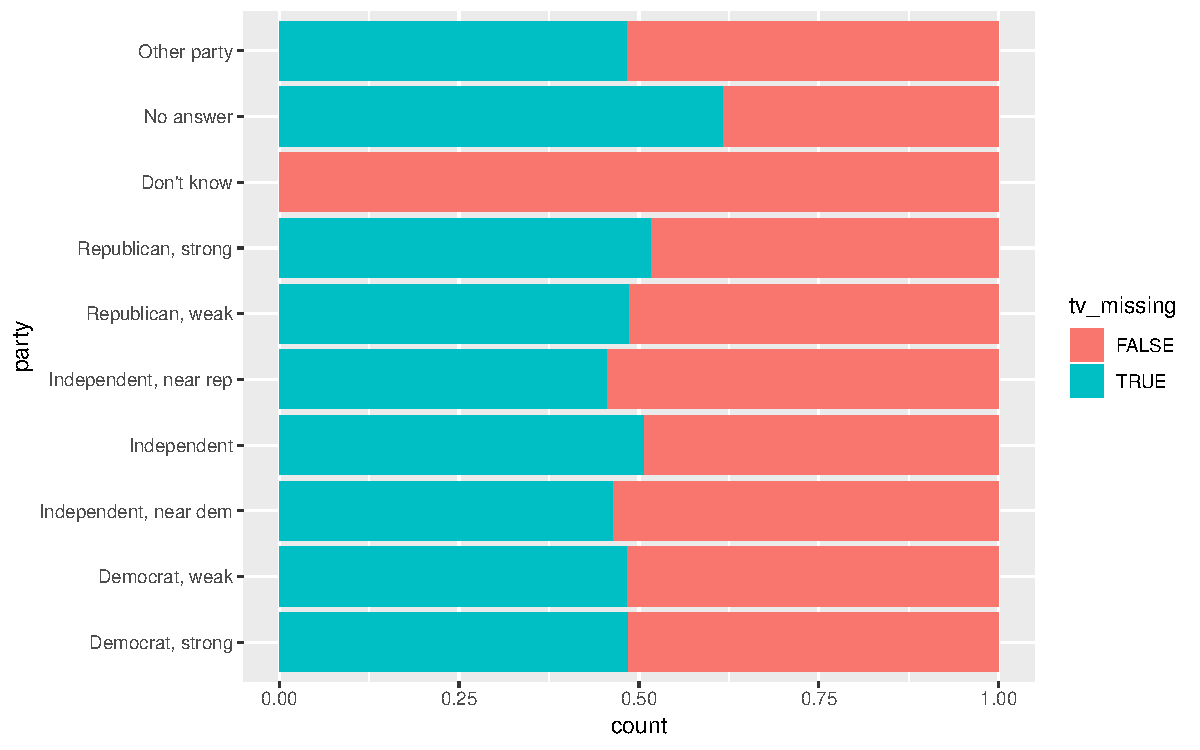
\includegraphics{cleaning_tutorial_files/figure-latex/unnamed-chunk-48-1}

As a final example, we can compare the missing of tv hours with a
continuous variable, let's say age. Are people who didn't report the
number of hours they watch tv generally older or younger? The boxplots
below don't show any difference.

\begin{Shaded}
\begin{Highlighting}[]
\NormalTok{survey_md }\OperatorTok\StringTok{ }\KeywordTok{ggplot}\NormalTok{(}\KeywordTok{aes}\NormalTok{(tv_missing, age, }\DataTypeTok{color =}\NormalTok{ tv_missing)) }\OperatorTok{+}\StringTok{ }
\StringTok{    }\KeywordTok{geom_boxplot}\NormalTok{()}
\end{Highlighting}
\end{Shaded}

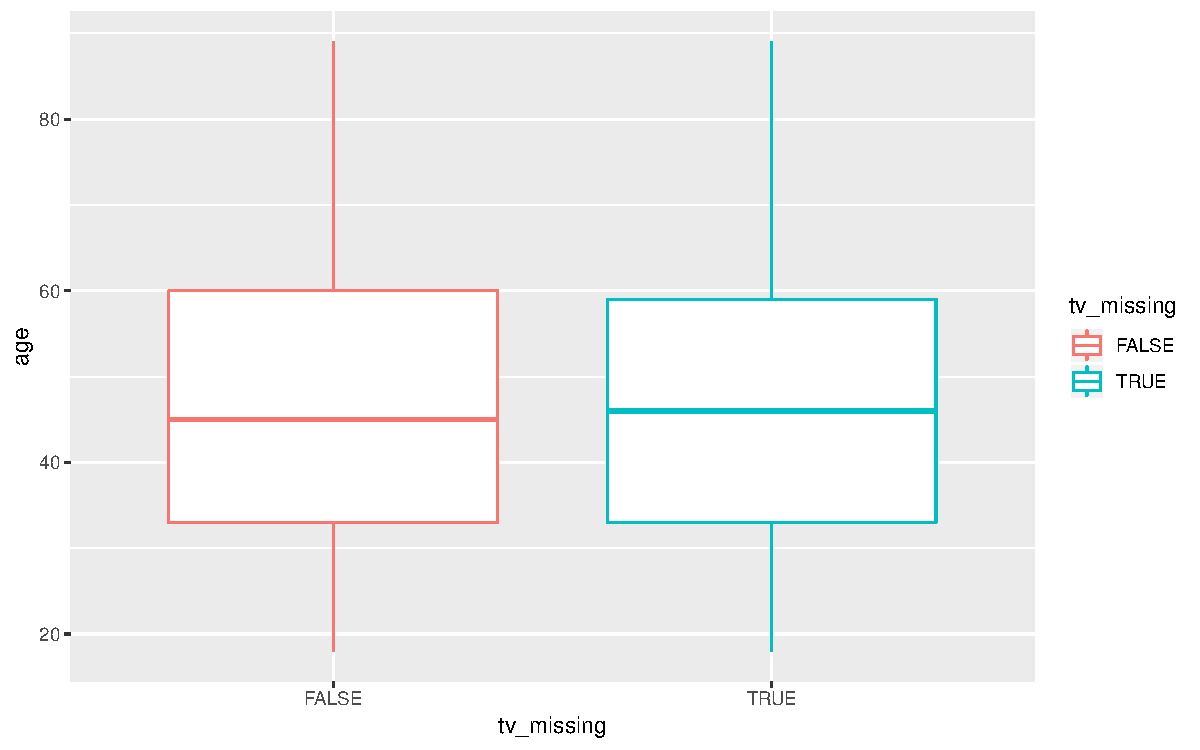
\includegraphics{cleaning_tutorial_files/figure-latex/unnamed-chunk-49-1}

How many comparisons you make for each variable where data is missing is
up to you -- but you have to gather reasonable evidence whether you
missing values are MAR, MCAR or NMAR.

\subsection{Working around missing
data}\label{working-around-missing-data}

While we will not see how to impute -- \emph{guess} -- missing values,
it is quite important to know how to work with them.

\subsubsection{Visualizations}\label{visualizations}

First, consider visualizations. When working with ggplot, missing values
will often be ignored automagically. For instance, if we try to create a
histogram of the age, ggplot will tell us that it ignored some missing
values through a warning.

\begin{Shaded}
\begin{Highlighting}[]
\NormalTok{survey }\OperatorTok\StringTok{ }\KeywordTok{ggplot}\NormalTok{(}\KeywordTok{aes}\NormalTok{(age)) }\OperatorTok{+}\StringTok{ }\KeywordTok{geom_histogram}\NormalTok{(}\DataTypeTok{binwidth =} \DecValTok{5}\NormalTok{, }
    \DataTypeTok{fill =} \StringTok{"dodgerblue4"}\NormalTok{, }\DataTypeTok{color =} \StringTok{"white"}\NormalTok{) }\OperatorTok{+}\StringTok{ }\KeywordTok{theme_light}\NormalTok{()}
\end{Highlighting}
\end{Shaded}

\begin{verbatim}
## Warning: Removed 76 rows containing non-finite
## values (stat_bin).
\end{verbatim}

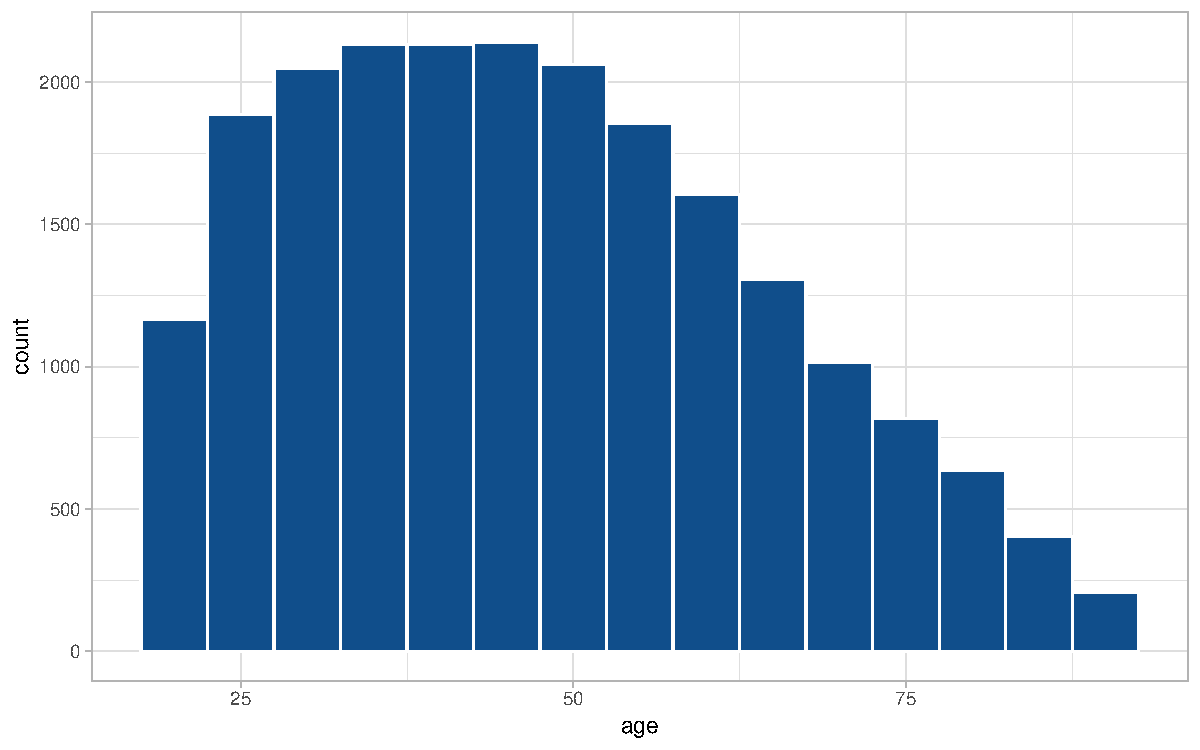
\includegraphics{cleaning_tutorial_files/figure-latex/unnamed-chunk-50-1}

The warning

\begin{Shaded}
\begin{Highlighting}[]
\NormalTok{## Warning: Removed 76 rows containing}
\NormalTok{## non-finite values (stat_bin).}
\end{Highlighting}
\end{Shaded}

tells us when and how many missing values are ignored.

In case that a categorical variable has missing values, NA will appear
as a seperate category. For example, consider the dataset survey2 (which
we will just use here as example), which has missing values for several
variables.

\begin{Shaded}
\begin{Highlighting}[]
\KeywordTok{summary}\NormalTok{(survey2)}
\end{Highlighting}
\end{Shaded}

\begin{verbatim}
##       age                  denomination 
##  Min.   :18.00   Not applicable  :9969  
##  1st Qu.:33.00   Other           :2519  
##  Median :46.00   No denomination :1664  
##  Mean   :47.18   Southern baptist:1515  
##  3rd Qu.:59.00   Baptist-dk which:1441  
##  Max.   :89.00   (Other)         :4151  
##  NA's   :288     NA's            : 224  
##           marital     
##  Divorced     : 3343  
##  Married      :10020  
##  Never married: 5364  
##  No answer    :   17  
##  Separated    :  733  
##  Widowed      : 1789  
##  NA's         :  217  
##                    party         race      
##  Independent          :4077   Black: 3098  
##  Democrat, weak       :3650   Other: 1934  
##  Democrat, strong     :3453   White:16223  
##  Republican, weak     :3000   NA's :  228  
##  Independent, near dem:2481                
##  (Other)              :4617                
##  NA's                 : 205                
##        religion           reported_income
##  Protestant:10734   $25000 or more:7306  
##  Catholic  : 5066   Not applicable:6973  
##  None      : 3480   $20000 - 24999:1272  
##  Christian :  684   $10000 - 14999:1156  
##  Jewish    :  383   $15000 - 19999:1037  
##  (Other)   :  906   (Other)       :3546  
##  NA's      :  230   NA's          : 193  
##     tv_hours          year     
##  Min.   :0.000   Min.   :2000  
##  1st Qu.:1.000   1st Qu.:2002  
##  Median :2.000   Median :2006  
##  Mean   :2.659   Mean   :2007  
##  3rd Qu.:4.000   3rd Qu.:2010  
##  Max.   :8.000   Max.   :2014  
##  NA's   :10609   NA's   :224
\end{verbatim}

Let's say we make a bar chart of the religion variable. The NA value
then appears as a seperate category and gets its own bar. Automatically,
this category will be plotted at the side of the others, not between
them.

\begin{Shaded}
\begin{Highlighting}[]
\NormalTok{survey2 }\OperatorTok\StringTok{ }\KeywordTok{ggplot}\NormalTok{(}\KeywordTok{aes}\NormalTok{(religion)) }\OperatorTok{+}\StringTok{ }\KeywordTok{geom_bar}\NormalTok{() }\OperatorTok{+}\StringTok{ }
\StringTok{    }\KeywordTok{coord_flip}\NormalTok{()}
\end{Highlighting}
\end{Shaded}

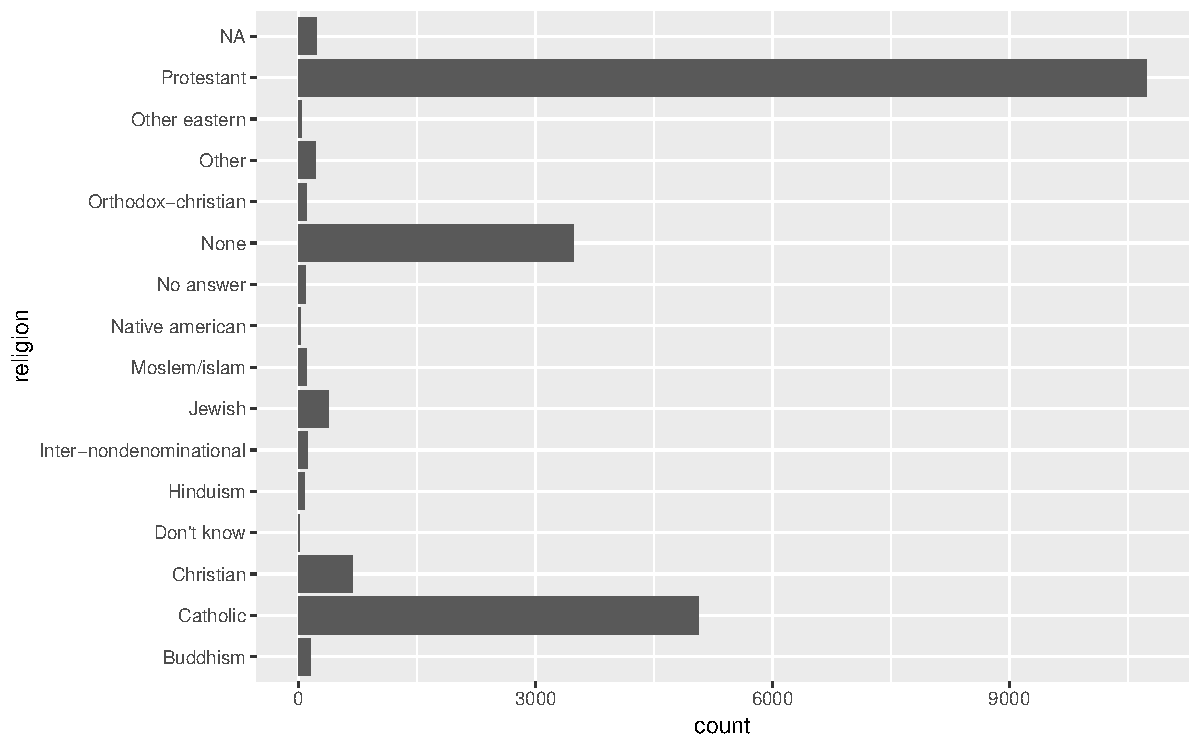
\includegraphics{cleaning_tutorial_files/figure-latex/unnamed-chunk-54-1}

As such, ggplot handles missing values without problem and quite
transparent. The same is not true when we go to numeric computations.

\subsubsection{Numerical analysis}\label{numerical-analysis}

Let's start with the good news. If we create a frequency table of a
categorical value with missing values, the NA's will be considered just
as any other value. For example, we can make a frequency table to
support the graph above for survey2.

\begin{Shaded}
\begin{Highlighting}[]
\NormalTok{survey2 }\OperatorTok\StringTok{ }\KeywordTok{group_by}\NormalTok{(religion) }\OperatorTok\StringTok{ }\KeywordTok{summarize}\NormalTok{(}\DataTypeTok{frequency =} \KeywordTok{n}\NormalTok{()) }\OperatorTok\StringTok{ }
\StringTok{    }\KeywordTok{mutate}\NormalTok{(}\DataTypeTok{relative_frequency =}\NormalTok{ frequency}\OperatorTok{/}\KeywordTok{sum}\NormalTok{(frequency)) }\OperatorTok\StringTok{ }
\StringTok{    }\KeywordTok{arrange}\NormalTok{(}\OperatorTok{-}\NormalTok{frequency) }\OperatorTok\StringTok{ }\NormalTok{pander}
\end{Highlighting}
\end{Shaded}

\begin{longtable}[]{@{}ccc@{}}
\toprule
\begin{minipage}[b]{0.33\columnwidth}\centering\strut
religion\strut
\end{minipage} & \begin{minipage}[b]{0.15\columnwidth}\centering\strut
frequency\strut
\end{minipage} & \begin{minipage}[b]{0.25\columnwidth}\centering\strut
relative\_frequency\strut
\end{minipage}\tabularnewline
\midrule
\endhead
\begin{minipage}[t]{0.33\columnwidth}\centering\strut
Protestant\strut
\end{minipage} & \begin{minipage}[t]{0.15\columnwidth}\centering\strut
10734\strut
\end{minipage} & \begin{minipage}[t]{0.25\columnwidth}\centering\strut
0.4997\strut
\end{minipage}\tabularnewline
\begin{minipage}[t]{0.33\columnwidth}\centering\strut
Catholic\strut
\end{minipage} & \begin{minipage}[t]{0.15\columnwidth}\centering\strut
5066\strut
\end{minipage} & \begin{minipage}[t]{0.25\columnwidth}\centering\strut
0.2358\strut
\end{minipage}\tabularnewline
\begin{minipage}[t]{0.33\columnwidth}\centering\strut
None\strut
\end{minipage} & \begin{minipage}[t]{0.15\columnwidth}\centering\strut
3480\strut
\end{minipage} & \begin{minipage}[t]{0.25\columnwidth}\centering\strut
0.162\strut
\end{minipage}\tabularnewline
\begin{minipage}[t]{0.33\columnwidth}\centering\strut
Christian\strut
\end{minipage} & \begin{minipage}[t]{0.15\columnwidth}\centering\strut
684\strut
\end{minipage} & \begin{minipage}[t]{0.25\columnwidth}\centering\strut
0.03184\strut
\end{minipage}\tabularnewline
\begin{minipage}[t]{0.33\columnwidth}\centering\strut
Jewish\strut
\end{minipage} & \begin{minipage}[t]{0.15\columnwidth}\centering\strut
383\strut
\end{minipage} & \begin{minipage}[t]{0.25\columnwidth}\centering\strut
0.01783\strut
\end{minipage}\tabularnewline
\begin{minipage}[t]{0.33\columnwidth}\centering\strut
NA\strut
\end{minipage} & \begin{minipage}[t]{0.15\columnwidth}\centering\strut
230\strut
\end{minipage} & \begin{minipage}[t]{0.25\columnwidth}\centering\strut
0.01071\strut
\end{minipage}\tabularnewline
\begin{minipage}[t]{0.33\columnwidth}\centering\strut
Other\strut
\end{minipage} & \begin{minipage}[t]{0.15\columnwidth}\centering\strut
220\strut
\end{minipage} & \begin{minipage}[t]{0.25\columnwidth}\centering\strut
0.01024\strut
\end{minipage}\tabularnewline
\begin{minipage}[t]{0.33\columnwidth}\centering\strut
Buddhism\strut
\end{minipage} & \begin{minipage}[t]{0.15\columnwidth}\centering\strut
147\strut
\end{minipage} & \begin{minipage}[t]{0.25\columnwidth}\centering\strut
0.006843\strut
\end{minipage}\tabularnewline
\begin{minipage}[t]{0.33\columnwidth}\centering\strut
Inter-nondenominational\strut
\end{minipage} & \begin{minipage}[t]{0.15\columnwidth}\centering\strut
108\strut
\end{minipage} & \begin{minipage}[t]{0.25\columnwidth}\centering\strut
0.005027\strut
\end{minipage}\tabularnewline
\begin{minipage}[t]{0.33\columnwidth}\centering\strut
Moslem/islam\strut
\end{minipage} & \begin{minipage}[t]{0.15\columnwidth}\centering\strut
104\strut
\end{minipage} & \begin{minipage}[t]{0.25\columnwidth}\centering\strut
0.004841\strut
\end{minipage}\tabularnewline
\begin{minipage}[t]{0.33\columnwidth}\centering\strut
Orthodox-christian\strut
\end{minipage} & \begin{minipage}[t]{0.15\columnwidth}\centering\strut
95\strut
\end{minipage} & \begin{minipage}[t]{0.25\columnwidth}\centering\strut
0.004422\strut
\end{minipage}\tabularnewline
\begin{minipage}[t]{0.33\columnwidth}\centering\strut
No answer\strut
\end{minipage} & \begin{minipage}[t]{0.15\columnwidth}\centering\strut
93\strut
\end{minipage} & \begin{minipage}[t]{0.25\columnwidth}\centering\strut
0.004329\strut
\end{minipage}\tabularnewline
\begin{minipage}[t]{0.33\columnwidth}\centering\strut
Hinduism\strut
\end{minipage} & \begin{minipage}[t]{0.15\columnwidth}\centering\strut
70\strut
\end{minipage} & \begin{minipage}[t]{0.25\columnwidth}\centering\strut
0.003258\strut
\end{minipage}\tabularnewline
\begin{minipage}[t]{0.33\columnwidth}\centering\strut
Other eastern\strut
\end{minipage} & \begin{minipage}[t]{0.15\columnwidth}\centering\strut
32\strut
\end{minipage} & \begin{minipage}[t]{0.25\columnwidth}\centering\strut
0.00149\strut
\end{minipage}\tabularnewline
\begin{minipage}[t]{0.33\columnwidth}\centering\strut
Native american\strut
\end{minipage} & \begin{minipage}[t]{0.15\columnwidth}\centering\strut
22\strut
\end{minipage} & \begin{minipage}[t]{0.25\columnwidth}\centering\strut
0.001024\strut
\end{minipage}\tabularnewline
\begin{minipage}[t]{0.33\columnwidth}\centering\strut
Don't know\strut
\end{minipage} & \begin{minipage}[t]{0.15\columnwidth}\centering\strut
15\strut
\end{minipage} & \begin{minipage}[t]{0.25\columnwidth}\centering\strut
0.0006982\strut
\end{minipage}\tabularnewline
\bottomrule
\end{longtable}

Unfortunately, the same is not true when we start to compute metrics for
centrality or spread. By design, when you apply a function on a vector
containing missing values, the function will return a missing value.
Consider the vector below, of which we want to know the mean and sum

\begin{Shaded}
\begin{Highlighting}[]
\NormalTok{x <-}\StringTok{ }\KeywordTok{c}\NormalTok{(}\DecValTok{5}\NormalTok{, }\DecValTok{6}\NormalTok{, }\DecValTok{12}\NormalTok{, }\OtherTok{NA}\NormalTok{, }\DecValTok{43}\NormalTok{)}
\KeywordTok{mean}\NormalTok{(x)}
\end{Highlighting}
\end{Shaded}

\begin{verbatim}
## [1] NA
\end{verbatim}

\begin{Shaded}
\begin{Highlighting}[]
\KeywordTok{sum}\NormalTok{(x)}
\end{Highlighting}
\end{Shaded}

\begin{verbatim}
## [1] NA
\end{verbatim}

Just as the warning we got when using ggplot with missing values, this
result is warning. It warns us that we want to compute something about a
vector which partly misses. However, the warning is quite strong here;
it doesn't give us anything we can use.

In order to circumvent this from happening, each of these functions has
a argument which is called \texttt{na.rm} -- meaning ``NA remove''. If
we say \texttt{na.rm\ =\ T}, missing values will be removed and ignored,
and the function will compute the result with the remaining value. Thus,

\begin{Shaded}
\begin{Highlighting}[]
\KeywordTok{mean}\NormalTok{(x, }\DataTypeTok{na.rm =}\NormalTok{ T)}
\end{Highlighting}
\end{Shaded}

\begin{verbatim}
## [1] 16.5
\end{verbatim}

\begin{Shaded}
\begin{Highlighting}[]
\KeywordTok{sum}\NormalTok{(x, }\DataTypeTok{na.rm =}\NormalTok{ T)}
\end{Highlighting}
\end{Shaded}

\begin{verbatim}
## [1] 66
\end{verbatim}

The fact that we have to explicitly state that we want to ignore missing
values is R's safety mechanism which prevents us from ignoring missing
values by accident.

Thus, if we want to compute measures of centrality and spread for, let's
say, age, we will need to use this argument if we want to come up with
anything.\footnote{Yes, we need to repeat this for each function we want
  to use, and no, there is no easier way.}

\begin{Shaded}
\begin{Highlighting}[]
\NormalTok{survey }\OperatorTok\StringTok{ }\KeywordTok{summarize}\NormalTok{(}\DataTypeTok{min =} \KeywordTok{min}\NormalTok{(age, }\DataTypeTok{na.rm =}\NormalTok{ T), }
    \DataTypeTok{mean =} \KeywordTok{mean}\NormalTok{(age, }\DataTypeTok{na.rm =}\NormalTok{ T), }\DataTypeTok{max =} \KeywordTok{max}\NormalTok{(age, }
        \DataTypeTok{na.rm =}\NormalTok{ T), }\DataTypeTok{iqr =} \KeywordTok{IQR}\NormalTok{(age, }\DataTypeTok{na.rm =}\NormalTok{ T))}
\end{Highlighting}
\end{Shaded}

\begin{verbatim}
## # A tibble: 1 x 4
##     min  mean   max   iqr
##   <dbl> <dbl> <dbl> <dbl>
## 1    18  47.2    89    26
\end{verbatim}

Finally, what happens when we want to compute correlations? For
instance, how is age and tv hours correlated. Both of these have missing
values. We could try the following:

\begin{Shaded}
\begin{Highlighting}[]
\NormalTok{survey }\OperatorTok\StringTok{ }\KeywordTok{select}\NormalTok{(age, tv_hours) }\OperatorTok\StringTok{ }\KeywordTok{cor}\NormalTok{(}\DataTypeTok{na.rm =}\NormalTok{ T)}
\end{Highlighting}
\end{Shaded}

\begin{verbatim}
## Error in cor(., na.rm = T): unused argument (na.rm = T)
\end{verbatim}

Oops, that was wishful thinking from my part. It seems that the
\texttt{na.rm} argument doesn't exist for the \texttt{cor} function. So
far for consistency in base R functions.

In order to compute correlations, we need to ensure that we only
consider rows without missing values. We can do this with the
\texttt{na.omit} function. This functions removes -- omits -- all rows
which have one or more missing values.

\begin{Shaded}
\begin{Highlighting}[]
\NormalTok{survey }\OperatorTok\StringTok{ }\KeywordTok{select}\NormalTok{(age, tv_hours) }\OperatorTok\StringTok{ }\KeywordTok{na.omit}\NormalTok{() }\OperatorTok\StringTok{ }
\StringTok{    }\KeywordTok{summary}\NormalTok{()}
\end{Highlighting}
\end{Shaded}

\begin{verbatim}
##       age           tv_hours    
##  Min.   :18.00   Min.   :0.000  
##  1st Qu.:33.00   1st Qu.:1.000  
##  Median :45.00   Median :2.000  
##  Mean   :47.13   Mean   :2.659  
##  3rd Qu.:60.00   3rd Qu.:4.000  
##  Max.   :89.00   Max.   :8.000
\end{verbatim}

Then, we can compute the correlation.

\begin{Shaded}
\begin{Highlighting}[]
\NormalTok{survey }\OperatorTok\StringTok{ }\KeywordTok{select}\NormalTok{(age, tv_hours) }\OperatorTok\StringTok{ }\KeywordTok{na.omit}\NormalTok{() }\OperatorTok\StringTok{ }
\StringTok{    }\KeywordTok{cor}\NormalTok{()}
\end{Highlighting}
\end{Shaded}

\begin{verbatim}
##                age  tv_hours
## age      1.0000000 0.1895392
## tv_hours 0.1895392 1.0000000
\end{verbatim}

The \texttt{na.omit} function can be somewhat dangerous and should only
be used in exceptional cases as these. It can make a huge difference if
we do it before select. Consider again the \texttt{survey2} dataset,
where all variables have some missing values.

This dataset has the following number of rows.

\begin{Shaded}
\begin{Highlighting}[]
\NormalTok{survey2 }\OperatorTok\StringTok{ }\KeywordTok{nrow}\NormalTok{()}
\end{Highlighting}
\end{Shaded}

\begin{verbatim}
## [1] 21483
\end{verbatim}

If we select age and tv hours, and remove rows with missing values, we
are left with the following number of rows

\begin{Shaded}
\begin{Highlighting}[]
\NormalTok{survey2 }\OperatorTok\StringTok{ }\KeywordTok{select}\NormalTok{(age, tv_hours) }\OperatorTok\StringTok{ }\KeywordTok{na.omit}\NormalTok{() }\OperatorTok\StringTok{ }
\StringTok{    }\KeywordTok{nrow}\NormalTok{()}
\end{Highlighting}
\end{Shaded}

\begin{verbatim}
## [1] 10727
\end{verbatim}

But, if we first remove rows with missing values, and then select the
two variables, we are only left with the following number of rows.

\begin{Shaded}
\begin{Highlighting}[]
\NormalTok{survey2 }\OperatorTok\StringTok{ }\KeywordTok{na.omit}\NormalTok{() }\OperatorTok\StringTok{ }\KeywordTok{select}\NormalTok{(age, tv_hours) }\OperatorTok\StringTok{ }
\StringTok{    }\KeywordTok{nrow}\NormalTok{()}
\end{Highlighting}
\end{Shaded}

\begin{verbatim}
## [1] 9989
\end{verbatim}

Do you see what's different? Have a good look. If we perform the removal
before the select, it will take into account missing values for ALL
variables. If we do the select first, it will only check for the
variables we retain. This nuance can make a huge difference in practice.
Using the \texttt{na.omit} function should always raise an alert in your
mind that directs you to be cautious.

In conclusion, it is advised to be cautious all the way when working
with missing value. And with those wise words, we end our cleaning
efforts, and proceed to transformations.

\chapter{Transforming Data}\label{transforming-data}

Whereas cleaning data is focussed on finding errors, transforming data
is about making it more easier to analyse. There are many ways to do so.

Firstly, we can remove the number of levels in a categorical variable,
preventing the plotting of too many different categories. Secondly, we
can also create new variables based on existing ones. The latter is also
called enriching data. Moreover, we can adjust variables to make them
easier to interpret. For example, using distances in km instead of miles
(or the other way around when your are British or American).
Furthermore, we might want to discretize continuous variables -- turning
them into categorical ones -- thereby enabling us to use other analyses
or visualizations. Finally, to conclude out tutorial, we will also
discuss some transformations which are useful when we are visualizing
data, most notably to order variables.

Many many things to do, so time to start.

\section{Discretization of continuous
variables}\label{discretization-of-continuous-variables}

Turning a continuous variable into a categorical one is called
discretization. Several functions to do this are provided by ggplot.

\begin{itemize}
\tightlist
\item
  \texttt{cut\_width}: creating intervals of a specific width
\item
  \texttt{cut\_interval}: creating a specific number of intervals of
  equal width
\item
  \texttt{cut\_number}: creating a specific number of interval with an
  equal number of observations.
\end{itemize}

For example, we can \emph{cut} tv hours into interval of width 4.
\footnote{The boundary argument is an optional argument to define where
  the interval should start.}

\begin{Shaded}
\begin{Highlighting}[]
\NormalTok{survey }\OperatorTok\StringTok{ }\KeywordTok{mutate}\NormalTok{(}\DataTypeTok{tv_hours =} \KeywordTok{cut_width}\NormalTok{(tv_hours, }
    \DataTypeTok{width =} \DecValTok{4}\NormalTok{, }\DataTypeTok{boundary =} \DecValTok{0}\NormalTok{)) }\OperatorTok\StringTok{ }\KeywordTok{count}\NormalTok{(tv_hours)}
\end{Highlighting}
\end{Shaded}

\begin{verbatim}
## # A tibble: 3 x 2
##   tv_hours     n
##   <fct>    <int>
## 1 [0,4]     9421
## 2 (4,8]     1553
## 3 <NA>     10509
\end{verbatim}

Alternatively, we can \emph{cut} tv hours into 4 intervals of equal
with.

\begin{Shaded}
\begin{Highlighting}[]
\NormalTok{survey }\OperatorTok\StringTok{ }\KeywordTok{mutate}\NormalTok{(}\DataTypeTok{tv_hours =} \KeywordTok{cut_interval}\NormalTok{(tv_hours, }
    \DataTypeTok{n =} \DecValTok{4}\NormalTok{)) }\OperatorTok\StringTok{ }\KeywordTok{count}\NormalTok{(tv_hours)}
\end{Highlighting}
\end{Shaded}

\begin{verbatim}
## # A tibble: 5 x 2
##   tv_hours     n
##   <fct>    <int>
## 1 [0,2]     6059
## 2 (2,4]     3362
## 3 (4,6]     1172
## 4 (6,8]      381
## 5 <NA>     10509
\end{verbatim}

Or, we can \emph{cut} tv hours into three intervals which contain an
equal number of observations.

\begin{Shaded}
\begin{Highlighting}[]
\NormalTok{survey }\OperatorTok\StringTok{ }\KeywordTok{mutate}\NormalTok{(}\DataTypeTok{tv_hours =} \KeywordTok{cut_number}\NormalTok{(tv_hours, }
    \DataTypeTok{n =} \DecValTok{3}\NormalTok{)) }\OperatorTok\StringTok{ }\KeywordTok{count}\NormalTok{(tv_hours)}
\end{Highlighting}
\end{Shaded}

\begin{verbatim}
## # A tibble: 4 x 2
##   tv_hours     n
##   <fct>    <int>
## 1 [0,2]     6059
## 2 (2,3]     1956
## 3 (3,8]     2959
## 4 <NA>     10509
\end{verbatim}

Here, it should be noted that the intervals do not contain the equal
amount of observations at all. This is because there are many
observations with a unique value wich cannot be split further. But
nevertheless, cut\_number will try its best, which will turn out better
if the values of the variable are more unique. For example, age lends
itself better for this:

\begin{Shaded}
\begin{Highlighting}[]
\NormalTok{survey }\OperatorTok\StringTok{ }\KeywordTok{mutate}\NormalTok{(}\DataTypeTok{age =} \KeywordTok{cut_number}\NormalTok{(age, }\DataTypeTok{n =} \DecValTok{5}\NormalTok{)) }\OperatorTok\StringTok{ }
\StringTok{    }\KeywordTok{count}\NormalTok{(age)}
\end{Highlighting}
\end{Shaded}

\begin{verbatim}
## # A tibble: 6 x 2
##   age         n
##   <fct>   <int>
## 1 [18,31]  4656
## 2 (31,41]  4305
## 3 (41,51]  4207
## 4 (51,63]  4149
## 5 (63,89]  4090
## 6 <NA>       76
\end{verbatim}

Each of the discritization functions allows us to modify the names of
the categories -- instead of the default interval notation by providing
a vector of names to the \texttt{labels} argument. For example

\begin{Shaded}
\begin{Highlighting}[]
\NormalTok{survey }\OperatorTok\StringTok{ }\KeywordTok{mutate}\NormalTok{(}\DataTypeTok{age_category =} \KeywordTok{cut_number}\NormalTok{(age, }
    \DataTypeTok{n =} \DecValTok{3}\NormalTok{, }\DataTypeTok{labels =} \KeywordTok{c}\NormalTok{(}\StringTok{"Young"}\NormalTok{, }\StringTok{"Middle-aged"}\NormalTok{, }
        \StringTok{"Old"}\NormalTok{))) }\OperatorTok\StringTok{ }\KeywordTok{group_by}\NormalTok{(age_category) }\OperatorTok\StringTok{ }
\StringTok{    }\KeywordTok{summarize}\NormalTok{(}\DataTypeTok{min =} \KeywordTok{min}\NormalTok{(age), }\DataTypeTok{max =} \KeywordTok{max}\NormalTok{(age), }
        \DataTypeTok{frequency =} \KeywordTok{n}\NormalTok{())}
\end{Highlighting}
\end{Shaded}

\begin{verbatim}
## # A tibble: 4 x 4
##   age_category   min   max frequency
##   <fct>        <dbl> <dbl>     <int>
## 1 Young           18    37      7234
## 2 Middle-aged     38    54      7117
## 3 Old             55    89      7056
## 4 <NA>            NA    NA        76
\end{verbatim}

In the last example we stored the discretized variable under a different
name. This is most advised, in order to not lose the original, detailed
data.

\section{Rescaling continuous
variables}\label{rescaling-continuous-variables}

When we have continuous variables, we can also adjust there scale. For
example, we can compute the percentage of tv hours per day by dividing
tv hours by 24.

\begin{Shaded}
\begin{Highlighting}[]
\NormalTok{survey }\OperatorTok\StringTok{ }\KeywordTok{mutate}\NormalTok{(}\DataTypeTok{tv_per_day =}\NormalTok{ tv_hours}\OperatorTok{/}\DecValTok{24}\NormalTok{) }\OperatorTok\StringTok{ }
\StringTok{    }\NormalTok{summary}
\end{Highlighting}
\end{Shaded}

\begin{verbatim}
##       year               marital     
##  Min.   :2000   Divorced     : 3383  
##  1st Qu.:2002   Married      :10117  
##  Median :2006   Never married: 5416  
##  Mean   :2007   No answer    :   17  
##  3rd Qu.:2010   Separated    :  743  
##  Max.   :2014   Widowed      : 1807  
##                                      
##       age           race      
##  Min.   :18.00   Black: 3129  
##  1st Qu.:33.00   Other: 1959  
##  Median :46.00   White:16395  
##  Mean   :47.18                
##  3rd Qu.:59.00                
##  Max.   :89.00                
##  NA's   :76                   
##        reported_income
##  $25000 or more:7363  
##  Not applicable:7043  
##  $20000 - 24999:1283  
##  $10000 - 14999:1168  
##  $15000 - 19999:1048  
##  Refused       : 975  
##  (Other)       :2603  
##                    party     
##  Independent          :4119  
##  Democrat, weak       :3690  
##  Democrat, strong     :3490  
##  Republican, weak     :3032  
##  Independent, near dem:2499  
##  Republican, strong   :2314  
##  (Other)              :2339  
##        religion               denomination  
##  Protestant:10846   Not applicable  :10072  
##  Catholic  : 5124   Other           : 2534  
##  None      : 3523   No denomination : 1683  
##  Christian :  689   Southern baptist: 1536  
##  Jewish    :  388   Baptist-dk which: 1457  
##  Other     :  224   United methodist: 1067  
##  (Other)   :  689   (Other)         : 3134  
##     tv_hours       tv_per_day   
##  Min.   :0.000   Min.   :0.000  
##  1st Qu.:1.000   1st Qu.:0.042  
##  Median :2.000   Median :0.083  
##  Mean   :2.659   Mean   :0.111  
##  3rd Qu.:4.000   3rd Qu.:0.167  
##  Max.   :8.000   Max.   :0.333  
##  NA's   :10509   NA's   :10509
\end{verbatim}

Other common transformations are:

\begin{itemize}
\tightlist
\item
  different currencies (euro vs dollar, etc.)
\item
  different measurement scales (miles vs km, inch vs cm, etc.)
\item
  different time zones or time units (on which more later).
\end{itemize}

\section{Adding calculated variables}\label{adding-calculated-variables}

The addition of calculated variables is similar to rescaling variables.
The only difference is that rescaling only relates to one variable,
while calculated variables can concern different variables.

For example, we can compute the year of birth for people in our data.

\begin{Shaded}
\begin{Highlighting}[]
\NormalTok{survey }\OperatorTok\StringTok{ }\KeywordTok{mutate}\NormalTok{(}\DataTypeTok{year_of_birth =}\NormalTok{ year }\OperatorTok{-}\StringTok{ }\NormalTok{age) }\OperatorTok\StringTok{ }
\StringTok{    }\KeywordTok{select}\NormalTok{(year, age, year_of_birth) }\OperatorTok\StringTok{ }\NormalTok{summary}
\end{Highlighting}
\end{Shaded}

\begin{verbatim}
##       year           age       
##  Min.   :2000   Min.   :18.00  
##  1st Qu.:2002   1st Qu.:33.00  
##  Median :2006   Median :46.00  
##  Mean   :2007   Mean   :47.18  
##  3rd Qu.:2010   3rd Qu.:59.00  
##  Max.   :2014   Max.   :89.00  
##                 NA's   :76     
##  year_of_birth 
##  Min.   :1911  
##  1st Qu.:1947  
##  Median :1960  
##  Mean   :1959  
##  3rd Qu.:1973  
##  Max.   :1996  
##  NA's   :76
\end{verbatim}

\section{Recode Categorical
Variables}\label{recode-categorical-variables-1}

When transforming categorical variables, our goal is often to reduce the
number of values. This can be done in different ways:

\begin{itemize}
\tightlist
\item
  combining values which are similar into a single value
\item
  combining infrequent values into a ``Various'' or ``Other'' value.
\end{itemize}

The first way can be done with \texttt{fct\_collapse}, which collapse
factor levels into a new level. The second can be achieved with
\texttt{fct\_lump}, which ``lumps'' together infrequent values.

\subsection{Collapsing factors}\label{collapsing-factors}

Collapsing a factor can be done as shown below. For each group of levels
that you want to collapse, you create a vector. Subsequently, you can
give each group a new name. \footnote{The attentative reader might have
  noticed a similarity between \texttt{fct\_collapse} and
  \texttt{fct\_recode}. Indeed, you could obtain the same result with
  the latter function, but you would have more typing work.} All levels
which you do not mentioned will be left untouched.

\begin{Shaded}
\begin{Highlighting}[]
\KeywordTok{fct_collapse}\NormalTok{(factor, }\DataTypeTok{new_group_1 =} \KeywordTok{c}\NormalTok{(}\StringTok{"old_level_1"}\NormalTok{, }
    \StringTok{"old_level_2"}\NormalTok{, }\StringTok{"..."}\NormalTok{), }\DataTypeTok{new_group_2 =} \KeywordTok{c}\NormalTok{(}\StringTok{"old_level_a"}\NormalTok{, }
    \StringTok{"old_level_b"}\NormalTok{, }\StringTok{"..."}\NormalTok{), ...)}
\end{Highlighting}
\end{Shaded}

In our survey data, we can collapse the party variable into different
groups: ``Democrat'',``Republican'',``Independent'' and ``Other''. We
save the new variable as party\_group.

\begin{Shaded}
\begin{Highlighting}[]
\NormalTok{survey <-}\StringTok{ }\NormalTok{survey }\OperatorTok\StringTok{ }\KeywordTok{mutate}\NormalTok{(}\DataTypeTok{party_group =} \KeywordTok{fct_collapse}\NormalTok{(party, }
    \DataTypeTok{Other =} \KeywordTok{c}\NormalTok{(}\StringTok{"No answer"}\NormalTok{, }\StringTok{"Don't know"}\NormalTok{, }\StringTok{"Other party"}\NormalTok{), }
    \DataTypeTok{Republican =} \KeywordTok{c}\NormalTok{(}\StringTok{"Republican, strong"}\NormalTok{, }\StringTok{"Republican, weak"}\NormalTok{), }
    \DataTypeTok{Independent =} \KeywordTok{c}\NormalTok{(}\StringTok{"Independent, near rep"}\NormalTok{, }\StringTok{"Independent"}\NormalTok{, }
        \StringTok{"Independent, near dem"}\NormalTok{), }\DataTypeTok{Democrat =} \KeywordTok{c}\NormalTok{(}\StringTok{"Democrat, weak"}\NormalTok{, }
        \StringTok{"Democrat, strong"}\NormalTok{)))}
\end{Highlighting}
\end{Shaded}

Transformations as these can be useful in there own right: reducing the
number of categories as in this plot.

\begin{Shaded}
\begin{Highlighting}[]
\NormalTok{survey }\OperatorTok\StringTok{ }\KeywordTok{ggplot}\NormalTok{(}\KeywordTok{aes}\NormalTok{(party_group)) }\OperatorTok{+}\StringTok{ }\KeywordTok{geom_bar}\NormalTok{() }\OperatorTok{+}\StringTok{ }
\StringTok{    }\KeywordTok{coord_flip}\NormalTok{()}
\end{Highlighting}
\end{Shaded}

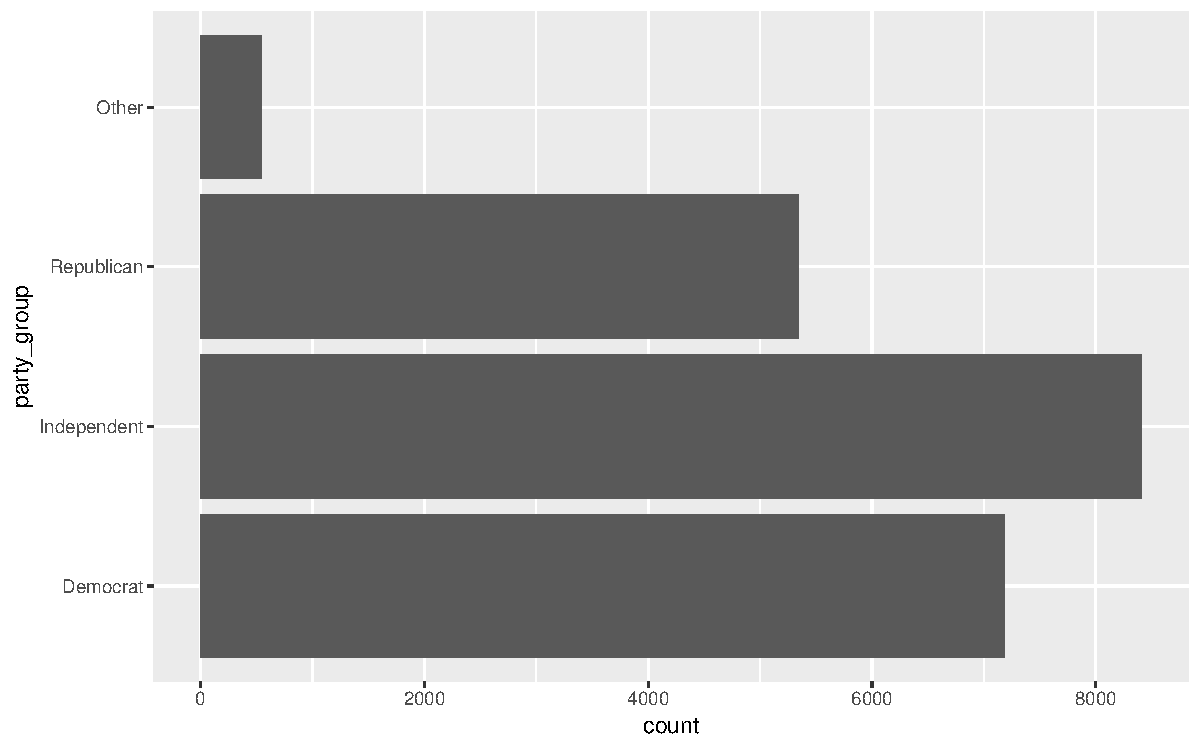
\includegraphics{cleaning_tutorial_files/figure-latex/unnamed-chunk-74-1}

But they can as well be used in combination with the original levels.
For example to improve visuals: \footnote{In this example, we use the
  scale\_fill\_tableau color scale from the package ggthemes to have a
  color scale where Democrats are blue and Republicans are red.
  Furthermore, we use fct\_rev to reverse the order of the factors.
  fct\_rev will be discussed in a few moments.}

\begin{Shaded}
\begin{Highlighting}[]
\KeywordTok{library}\NormalTok{(ggthemes)}
\NormalTok{survey }\OperatorTok\StringTok{ }\KeywordTok{ggplot}\NormalTok{(}\KeywordTok{aes}\NormalTok{(party, }\DataTypeTok{fill =}\NormalTok{ party_group)) }\OperatorTok{+}\StringTok{ }
\StringTok{    }\KeywordTok{geom_bar}\NormalTok{() }\OperatorTok{+}\StringTok{ }\KeywordTok{facet_grid}\NormalTok{(}\KeywordTok{fct_rev}\NormalTok{(party_group) }\OperatorTok{~}\StringTok{ }
\StringTok{    }\NormalTok{., }\DataTypeTok{scales =} \StringTok{"free"}\NormalTok{, }\DataTypeTok{space =} \StringTok{"free"}\NormalTok{) }\OperatorTok{+}\StringTok{ }\KeywordTok{coord_flip}\NormalTok{() }\OperatorTok{+}\StringTok{ }
\StringTok{    }\KeywordTok{scale_fill_tableau}\NormalTok{()}
\end{Highlighting}
\end{Shaded}

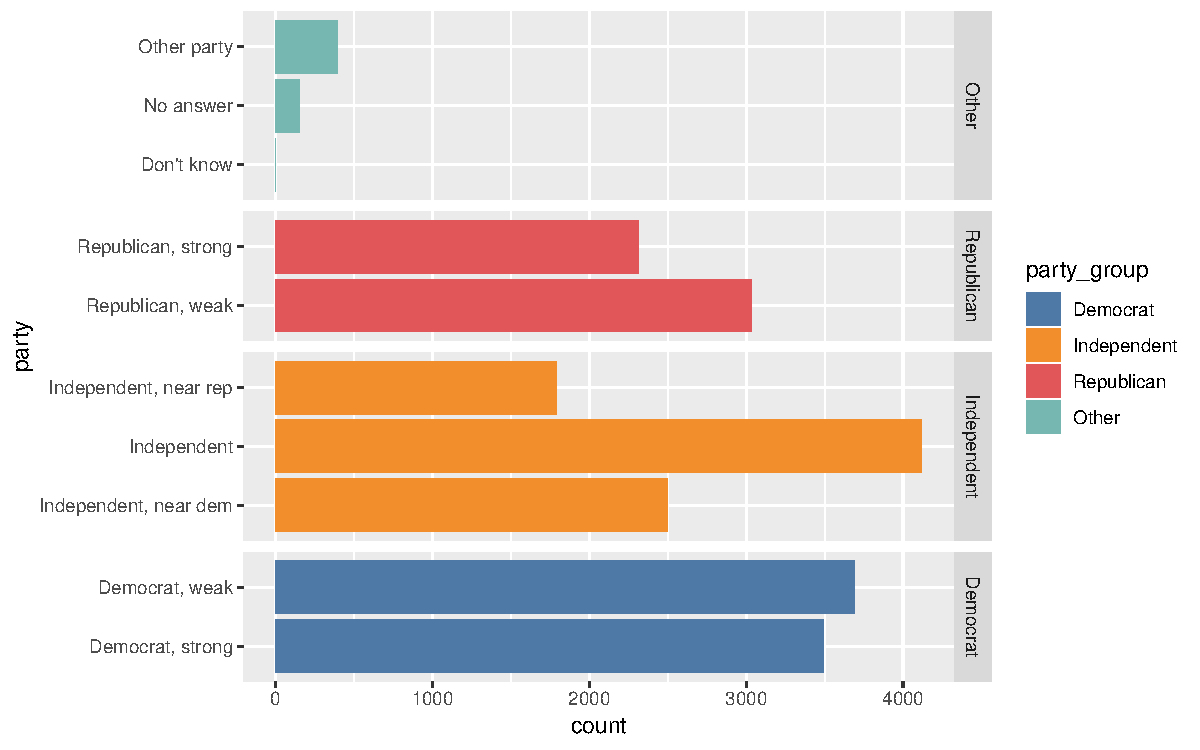
\includegraphics{cleaning_tutorial_files/figure-latex/unnamed-chunk-75-1}

Alternatively, we can use fct\_lump to create an other category. For
example, take a look at the religions.

\begin{Shaded}
\begin{Highlighting}[]
\NormalTok{survey }\OperatorTok\StringTok{ }\KeywordTok{count}\NormalTok{(religion)}
\end{Highlighting}
\end{Shaded}

\begin{verbatim}
## # A tibble: 15 x 2
##    religion                    n
##    <fct>                   <int>
##  1 Buddhism                  147
##  2 Catholic                 5124
##  3 Christian                 689
##  4 Don't know                 15
##  5 Hinduism                   71
##  6 Inter-nondenominational   109
##  7 Jewish                    388
##  8 Moslem/islam              104
##  9 Native american            23
## 10 No answer                  93
## 11 None                     3523
## 12 Orthodox-christian         95
## 13 Other                     224
## 14 Other eastern              32
## 15 Protestant              10846
\end{verbatim}

Let's say we want to keep only the 5 most frequent religions. We can do
this as follows.

\begin{Shaded}
\begin{Highlighting}[]
\NormalTok{survey }\OperatorTok\StringTok{ }\KeywordTok{mutate}\NormalTok{(}\DataTypeTok{religion =} \KeywordTok{fct_lump}\NormalTok{(religion, }
    \DataTypeTok{n =} \DecValTok{5}\NormalTok{)) }\OperatorTok\StringTok{ }\KeywordTok{count}\NormalTok{(religion)}
\end{Highlighting}
\end{Shaded}

\begin{verbatim}
## # A tibble: 6 x 2
##   religion       n
##   <fct>      <int>
## 1 Catholic    5124
## 2 Christian    689
## 3 Jewish       388
## 4 None        3523
## 5 Protestant 10846
## 6 Other        913
\end{verbatim}

The ``Other'' label can be changed as you like.

\begin{Shaded}
\begin{Highlighting}[]
\NormalTok{survey }\OperatorTok\StringTok{ }\KeywordTok{mutate}\NormalTok{(}\DataTypeTok{religion =} \KeywordTok{fct_lump}\NormalTok{(religion, }
    \DataTypeTok{n =} \DecValTok{5}\NormalTok{, }\DataTypeTok{other_level =} \StringTok{"Other religions"}\NormalTok{)) }\OperatorTok\StringTok{ }
\StringTok{    }\KeywordTok{count}\NormalTok{(religion)}
\end{Highlighting}
\end{Shaded}

\begin{verbatim}
## # A tibble: 6 x 2
##   religion            n
##   <fct>           <int>
## 1 Catholic         5124
## 2 Christian         689
## 3 Jewish            388
## 4 None             3523
## 5 Protestant      10846
## 6 Other religions   913
\end{verbatim}

Instead of specifying the number of levels to retain, you can also
specify a minimal relative frequenties using the \texttt{prop} argument.

\begin{Shaded}
\begin{Highlighting}[]
\NormalTok{survey }\OperatorTok\StringTok{ }\KeywordTok{mutate}\NormalTok{(}\DataTypeTok{religion =} \KeywordTok{fct_lump}\NormalTok{(religion, }
    \DataTypeTok{prop =} \FloatTok{0.02}\NormalTok{)) }\OperatorTok\StringTok{ }\KeywordTok{count}\NormalTok{(religion)}
\end{Highlighting}
\end{Shaded}

\begin{verbatim}
## # A tibble: 5 x 2
##   religion       n
##   <fct>      <int>
## 1 Catholic    5124
## 2 Christian    689
## 3 None        3523
## 4 Protestant 10846
## 5 Other       1301
\end{verbatim}

Even more so than cleaning, all the transformations we have seen are
very iterative in nature, and their use can be for specific analyses
only. For example, we might want to lump infrequent religions to make a
bar chart without to many bars -- but we probably don't want to remove
infrequent religions all the way. Transformations will thus often happen
in the build-up towards a chart or table, and not permanently saved in
the data. This is especially true for the last functions we will discuss
here: reordering functions.

\chapter{Using transformations in
visualizations.}\label{using-transformations-in-visualizations.}

When visualization categorical variables, we often want to change to
order of levels according to frequency or based on another variable. We
already saw \texttt{fct\_relevel} to manually reorder levels, but its
not very suited to automatically reorder levels. For this, we will use
two new functions: fct\_infreq and fct\_reorder.

We start with the following graph.

\begin{Shaded}
\begin{Highlighting}[]
\NormalTok{survey }\OperatorTok\StringTok{ }\KeywordTok{ggplot}\NormalTok{(}\KeywordTok{aes}\NormalTok{(religion)) }\OperatorTok{+}\StringTok{ }\KeywordTok{geom_bar}\NormalTok{() }\OperatorTok{+}\StringTok{ }
\StringTok{    }\KeywordTok{coord_flip}\NormalTok{()}
\end{Highlighting}
\end{Shaded}

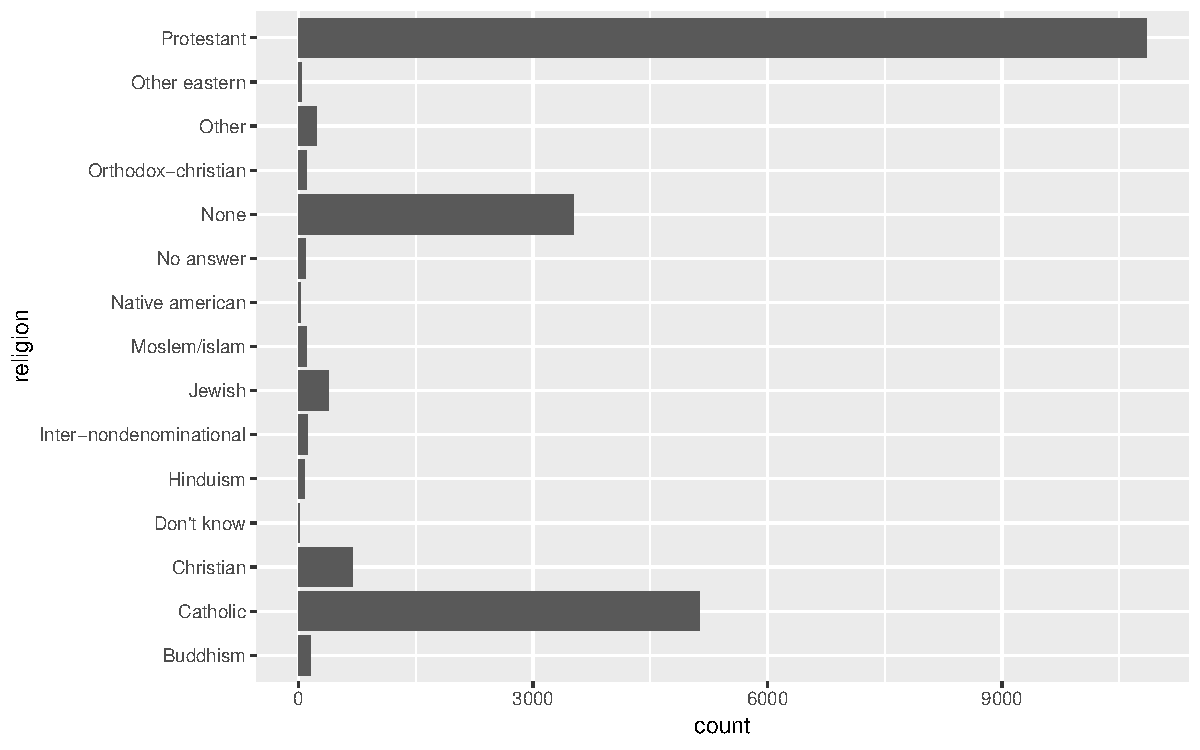
\includegraphics{cleaning_tutorial_files/figure-latex/unnamed-chunk-80-1}

A factor can be ordered based on the (in)frequency of each level using
the fct\_infreq function. Its use is simple. We can choose to add the
function directly within ggplot, or to update the religion variable
using mutate in advance of plotting.

\begin{Shaded}
\begin{Highlighting}[]
\NormalTok{survey }\OperatorTok\StringTok{ }\KeywordTok{ggplot}\NormalTok{(}\KeywordTok{aes}\NormalTok{(}\KeywordTok{fct_infreq}\NormalTok{(religion))) }\OperatorTok{+}\StringTok{ }
\StringTok{    }\KeywordTok{geom_bar}\NormalTok{() }\OperatorTok{+}\StringTok{ }\KeywordTok{coord_flip}\NormalTok{()}
\end{Highlighting}
\end{Shaded}

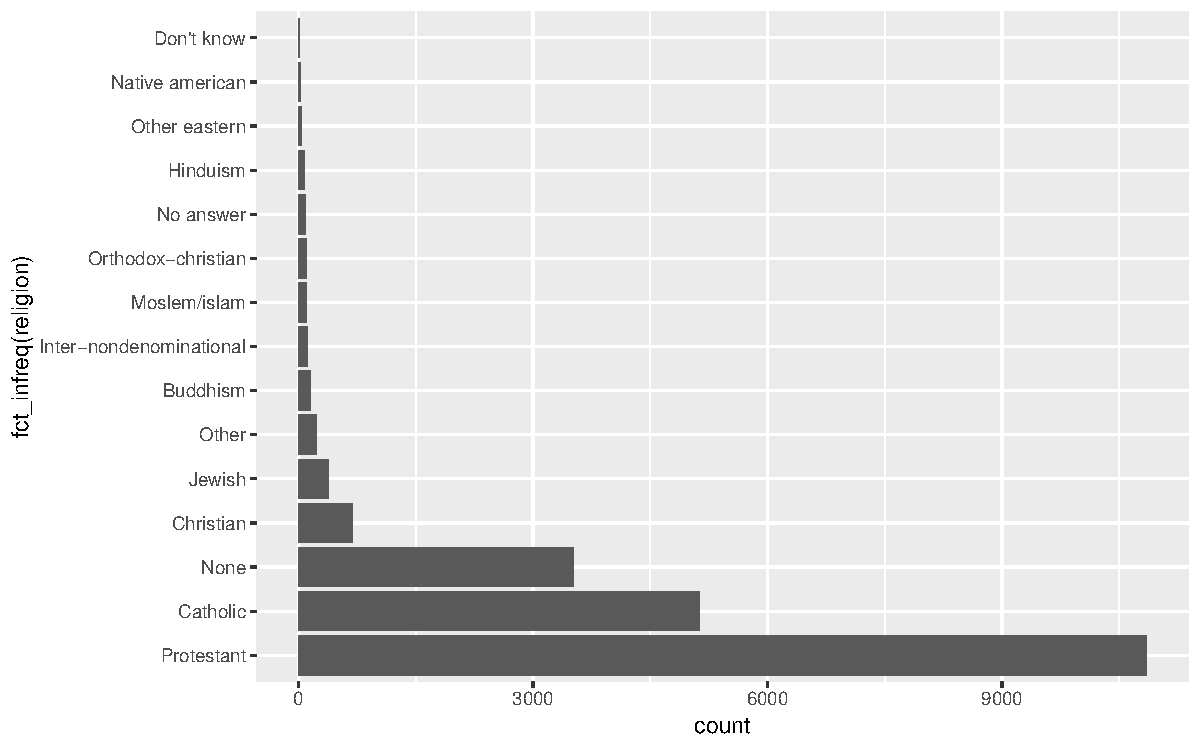
\includegraphics{cleaning_tutorial_files/figure-latex/unnamed-chunk-81-1}

\texttt{fct\_infreq} will count for each of the levels -- religions in
this case -- how often it occurs, and reorder the levels accordingly.
Now, suppose that we don't want absolute frequencies like in the last
plot, but relative. In that case, we need to compute them ourselves and
use \texttt{geom\_col}.

\begin{Shaded}
\begin{Highlighting}[]
\NormalTok{survey }\OperatorTok\StringTok{ }\KeywordTok{group_by}\NormalTok{(religion) }\OperatorTok\StringTok{ }\KeywordTok{summarise}\NormalTok{(}\DataTypeTok{freq =} \KeywordTok{n}\NormalTok{()) }\OperatorTok\StringTok{ }
\StringTok{    }\KeywordTok{mutate}\NormalTok{(}\DataTypeTok{rel_freq =}\NormalTok{ freq}\OperatorTok{/}\KeywordTok{sum}\NormalTok{(freq)) }\OperatorTok\StringTok{ }\KeywordTok{ggplot}\NormalTok{(}\KeywordTok{aes}\NormalTok{(}\DataTypeTok{x =}\NormalTok{ religion, }
    \DataTypeTok{y =}\NormalTok{ rel_freq)) }\OperatorTok{+}\StringTok{ }\KeywordTok{geom_col}\NormalTok{() }\OperatorTok{+}\StringTok{ }\KeywordTok{coord_flip}\NormalTok{()}
\end{Highlighting}
\end{Shaded}

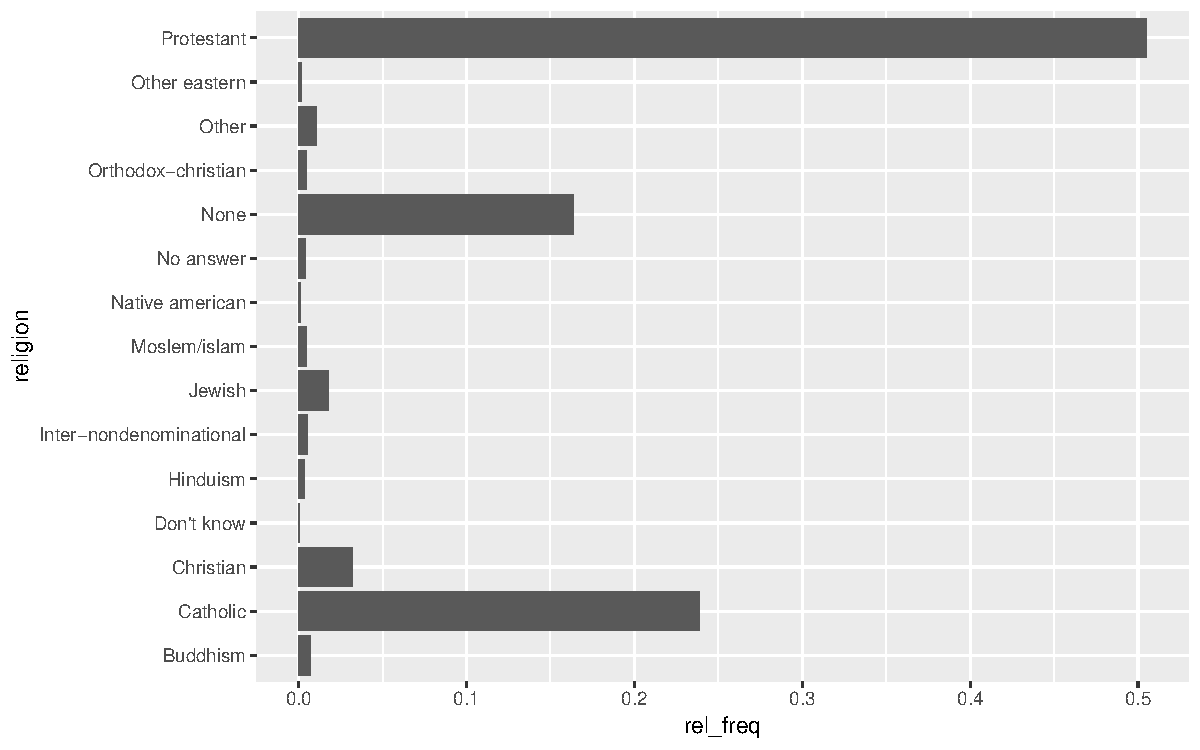
\includegraphics{cleaning_tutorial_files/figure-latex/unnamed-chunk-82-1}

We now can see read the relative frequencies from the chart. Now let's
order the bars once more.

\begin{Shaded}
\begin{Highlighting}[]
\NormalTok{survey }\OperatorTok\StringTok{ }\KeywordTok{group_by}\NormalTok{(religion) }\OperatorTok\StringTok{ }\KeywordTok{summarise}\NormalTok{(}\DataTypeTok{freq =} \KeywordTok{n}\NormalTok{()) }\OperatorTok\StringTok{ }
\StringTok{    }\KeywordTok{mutate}\NormalTok{(}\DataTypeTok{rel_freq =}\NormalTok{ freq}\OperatorTok{/}\KeywordTok{sum}\NormalTok{(freq)) }\OperatorTok\StringTok{ }\KeywordTok{ggplot}\NormalTok{(}\KeywordTok{aes}\NormalTok{(}\DataTypeTok{x =} \KeywordTok{fct_infreq}\NormalTok{(religion), }
    \DataTypeTok{y =}\NormalTok{ rel_freq)) }\OperatorTok{+}\StringTok{ }\KeywordTok{geom_col}\NormalTok{() }\OperatorTok{+}\StringTok{ }\KeywordTok{coord_flip}\NormalTok{()}
\end{Highlighting}
\end{Shaded}

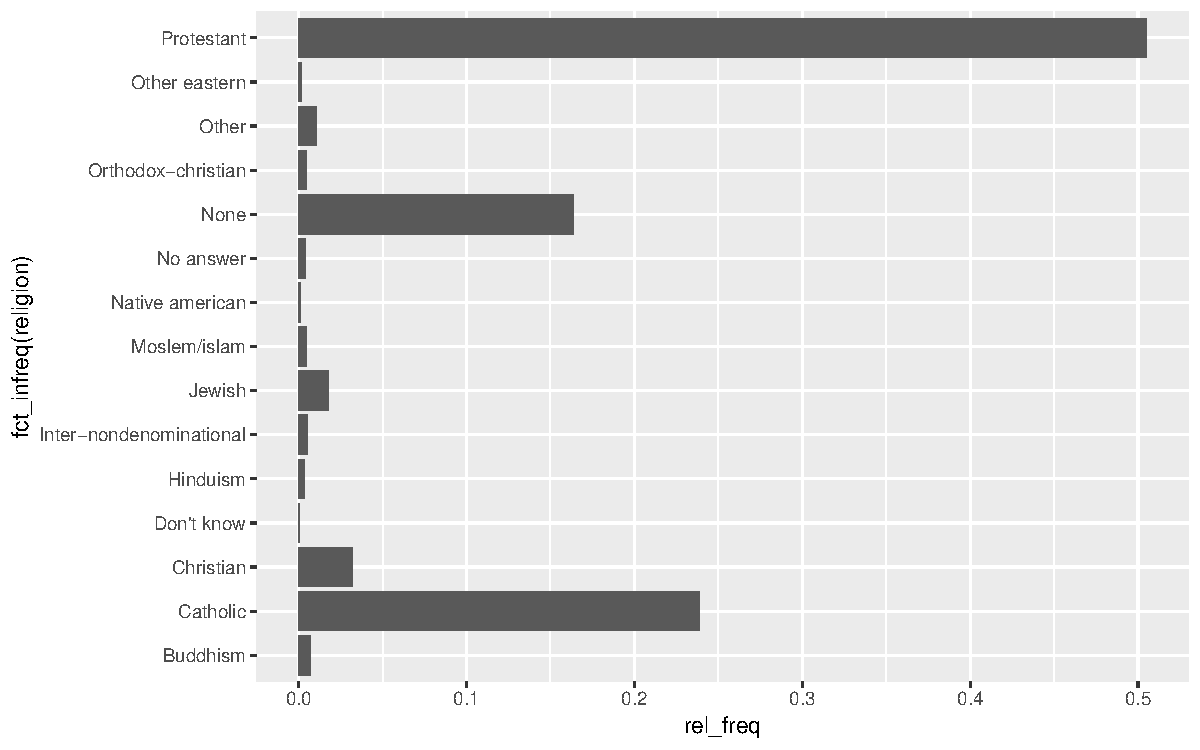
\includegraphics{cleaning_tutorial_files/figure-latex/unnamed-chunk-83-1}

Oops, that didn't seem to work. Why not? Let's look at the data we gave
to ggplot.

\begin{Shaded}
\begin{Highlighting}[]
\NormalTok{survey }\OperatorTok\StringTok{ }\KeywordTok{group_by}\NormalTok{(religion) }\OperatorTok\StringTok{ }\KeywordTok{summarise}\NormalTok{(}\DataTypeTok{freq =} \KeywordTok{n}\NormalTok{()) }\OperatorTok\StringTok{ }
\StringTok{    }\KeywordTok{mutate}\NormalTok{(}\DataTypeTok{rel_freq =}\NormalTok{ freq}\OperatorTok{/}\KeywordTok{sum}\NormalTok{(freq))}
\end{Highlighting}
\end{Shaded}

\begin{verbatim}
## # A tibble: 15 x 3
##    religion                 freq rel_freq
##    <fct>                   <int>    <dbl>
##  1 Buddhism                  147 0.00684 
##  2 Catholic                 5124 0.239   
##  3 Christian                 689 0.0321  
##  4 Don't know                 15 0.000698
##  5 Hinduism                   71 0.00330 
##  6 Inter-nondenominational   109 0.00507 
##  7 Jewish                    388 0.0181  
##  8 Moslem/islam              104 0.00484 
##  9 Native american            23 0.00107 
## 10 No answer                  93 0.00433 
## 11 None                     3523 0.164   
## 12 Orthodox-christian         95 0.00442 
## 13 Other                     224 0.0104  
## 14 Other eastern              32 0.00149 
## 15 Protestant              10846 0.505
\end{verbatim}

The data -- a frequency table -- contains one row for each religion.
When we use \texttt{fct\_infreq} on this table, all religions appear
once, so there are all equally frequent. \texttt{fct\_infreq} implicitly
tries to compute frequencies, but we already did that. As a result, the
ordering failed. It is similar to using \texttt{geom\_bar} based on a
frequency table -- we are trying to compute the frequencies twice, which
results in unintended plots.

So, what can we do instead? Well, we want to order the religions based
on frequency. That shouldn't be hard, because the frequency is already
there. The function \texttt{fct\_reorder} can help us. In contrast to
\texttt{fct\_infreq} it will use a second variable we provide to order
the factor. Thus:

\begin{Shaded}
\begin{Highlighting}[]
\NormalTok{survey }\OperatorTok\StringTok{ }\KeywordTok{group_by}\NormalTok{(religion) }\OperatorTok\StringTok{ }\KeywordTok{summarise}\NormalTok{(}\DataTypeTok{freq =} \KeywordTok{n}\NormalTok{()) }\OperatorTok\StringTok{ }
\StringTok{    }\KeywordTok{mutate}\NormalTok{(}\DataTypeTok{rel_freq =}\NormalTok{ freq}\OperatorTok{/}\KeywordTok{sum}\NormalTok{(freq)) }\OperatorTok\StringTok{ }\KeywordTok{ggplot}\NormalTok{(}\KeywordTok{aes}\NormalTok{(}\DataTypeTok{x =} \KeywordTok{fct_reorder}\NormalTok{(religion, }
\NormalTok{    rel_freq), }\DataTypeTok{y =}\NormalTok{ rel_freq)) }\OperatorTok{+}\StringTok{ }\KeywordTok{geom_col}\NormalTok{() }\OperatorTok{+}\StringTok{ }\KeywordTok{coord_flip}\NormalTok{()}
\end{Highlighting}
\end{Shaded}

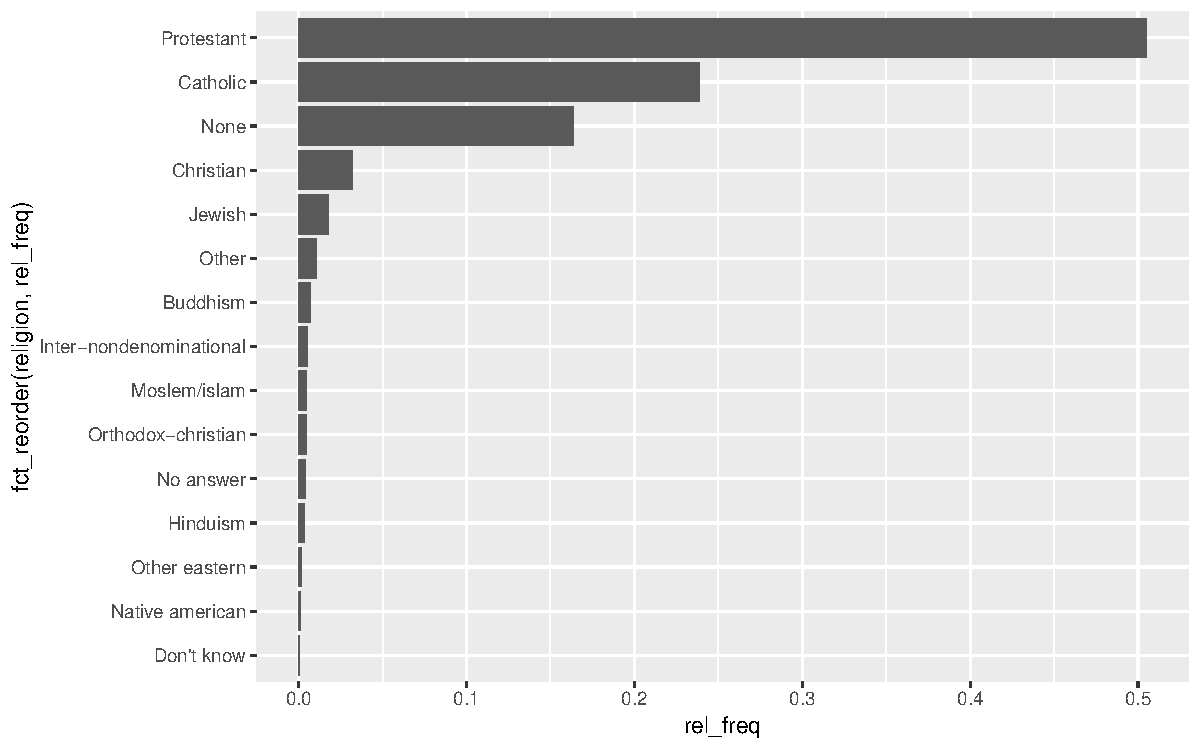
\includegraphics{cleaning_tutorial_files/figure-latex/unnamed-chunk-85-1}

Note how we refer to rel\_freq twice: once to order, and once to use as
y-axis. Also note that the order of the bars is reversed:
\texttt{fct\_infreq} will always order from most to least frequent,
while our current configuration with \texttt{fct\_reorder} is ordering
from least to most frequent. We can simply change it using desc(), as we
have done before.

\begin{Shaded}
\begin{Highlighting}[]
\NormalTok{survey }\OperatorTok\StringTok{ }\KeywordTok{group_by}\NormalTok{(religion) }\OperatorTok\StringTok{ }\KeywordTok{summarise}\NormalTok{(}\DataTypeTok{freq =} \KeywordTok{n}\NormalTok{()) }\OperatorTok\StringTok{ }
\StringTok{    }\KeywordTok{mutate}\NormalTok{(}\DataTypeTok{rel_freq =}\NormalTok{ freq}\OperatorTok{/}\KeywordTok{sum}\NormalTok{(freq)) }\OperatorTok\StringTok{ }\KeywordTok{ggplot}\NormalTok{(}\KeywordTok{aes}\NormalTok{(}\DataTypeTok{x =} \KeywordTok{fct_reorder}\NormalTok{(religion, }
    \KeywordTok{desc}\NormalTok{(rel_freq)), }\DataTypeTok{y =}\NormalTok{ rel_freq)) }\OperatorTok{+}\StringTok{ }\KeywordTok{geom_col}\NormalTok{() }\OperatorTok{+}\StringTok{ }
\StringTok{    }\KeywordTok{coord_flip}\NormalTok{()}
\end{Highlighting}
\end{Shaded}

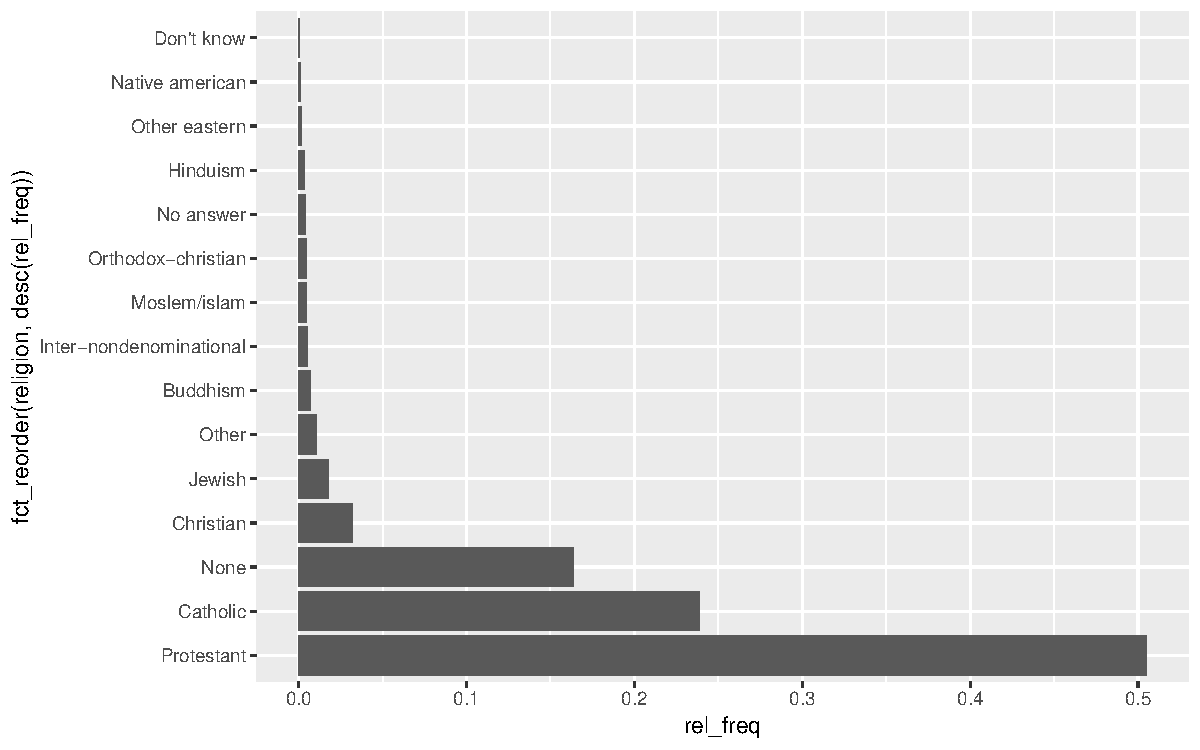
\includegraphics{cleaning_tutorial_files/figure-latex/unnamed-chunk-86-1}

Alternatively, we can use the \texttt{fct\_rev} function: this function
will reverse the order of a factor. For example, we can reverse the
order made by \texttt{fct\_infreq}.

\begin{Shaded}
\begin{Highlighting}[]
\NormalTok{survey }\OperatorTok\StringTok{ }\KeywordTok{ggplot}\NormalTok{(}\KeywordTok{aes}\NormalTok{(}\KeywordTok{fct_rev}\NormalTok{(}\KeywordTok{fct_infreq}\NormalTok{(religion)))) }\OperatorTok{+}\StringTok{ }
\StringTok{    }\KeywordTok{geom_bar}\NormalTok{() }\OperatorTok{+}\StringTok{ }\KeywordTok{coord_flip}\NormalTok{()}
\end{Highlighting}
\end{Shaded}

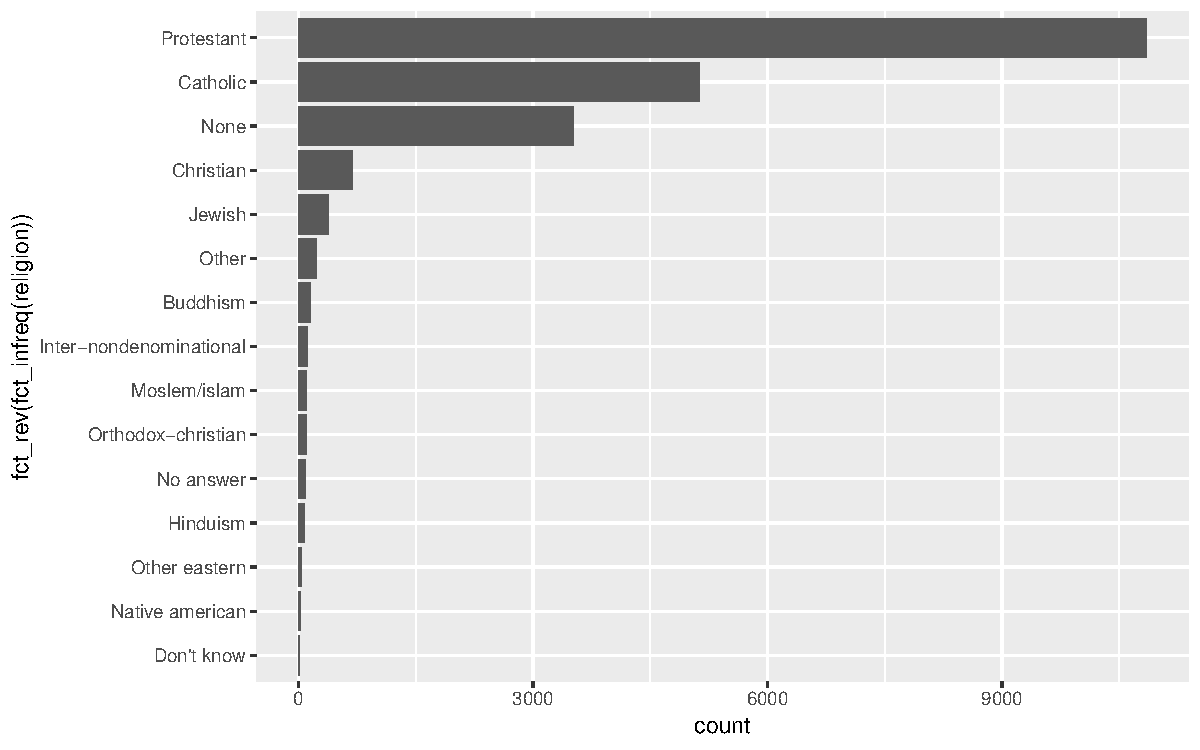
\includegraphics{cleaning_tutorial_files/figure-latex/unnamed-chunk-87-1}

Thus, summarizing:

\begin{itemize}
\tightlist
\item
  \texttt{fct\_infreq(f)}: reorder the levels of factor f from most to
  least frequent
\item
  \texttt{fct\_reorder(f,\ x)}: reorder the levels of factor f according
  to variable x
\item
  \texttt{fct\_rev(f)}: reverse the order of the levels of factor f
\end{itemize}

In general, you should use \texttt{fct\_infreq} only on the original
data, and when you have a frequency table as input to ggplot, you should
use \texttt{fct\_reorder}.

However, there is one more thing we need to cover.
\texttt{fct\_reorder(f,x)} can reorder on any variable x, not just
frequency. For example, look at the following plot.

\begin{Shaded}
\begin{Highlighting}[]
\NormalTok{survey }\OperatorTok\StringTok{ }\KeywordTok{ggplot}\NormalTok{(}\KeywordTok{aes}\NormalTok{(marital, age)) }\OperatorTok{+}\StringTok{ }\KeywordTok{geom_boxplot}\NormalTok{()}
\end{Highlighting}
\end{Shaded}

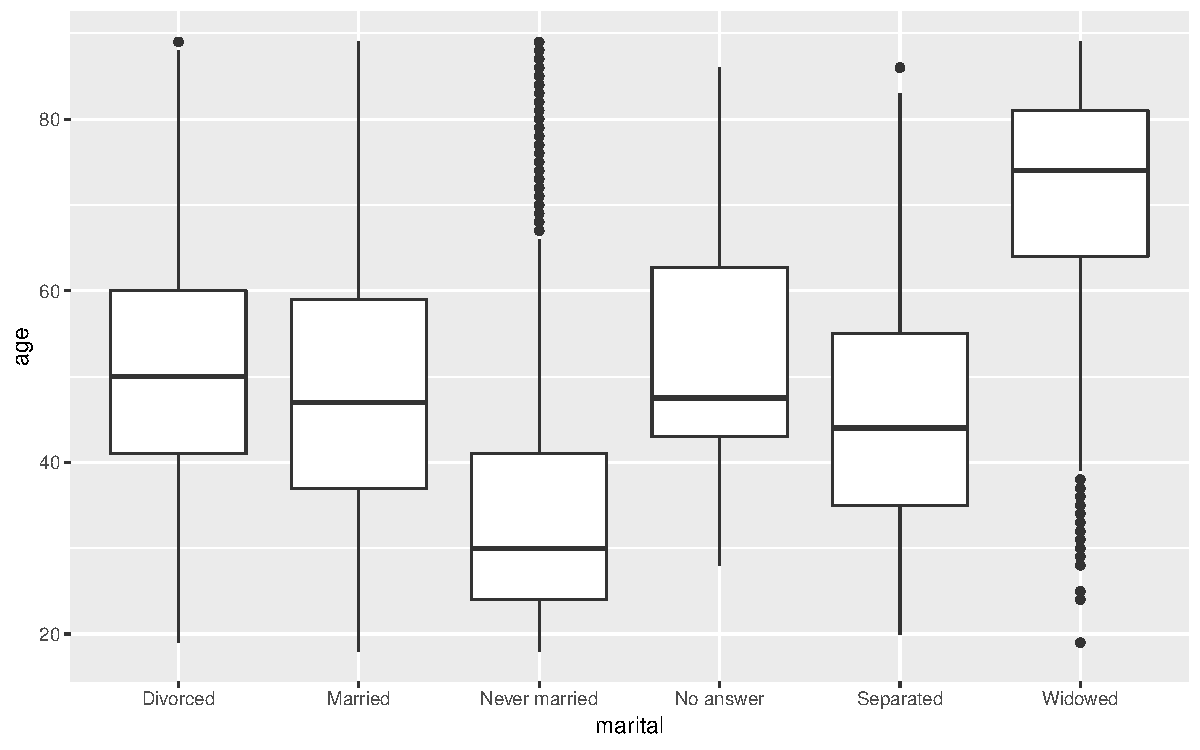
\includegraphics{cleaning_tutorial_files/figure-latex/unnamed-chunk-88-1}

This plot shows the distribution of age for different marital statuses.
Let's say we want to sort these boxplots according to age. We use
\texttt{fct\_reorder} just as we did before.

\begin{Shaded}
\begin{Highlighting}[]
\NormalTok{survey }\OperatorTok\StringTok{ }\KeywordTok{ggplot}\NormalTok{(}\KeywordTok{aes}\NormalTok{(}\KeywordTok{fct_reorder}\NormalTok{(marital, age), }
\NormalTok{    age)) }\OperatorTok{+}\StringTok{ }\KeywordTok{geom_boxplot}\NormalTok{()}
\end{Highlighting}
\end{Shaded}

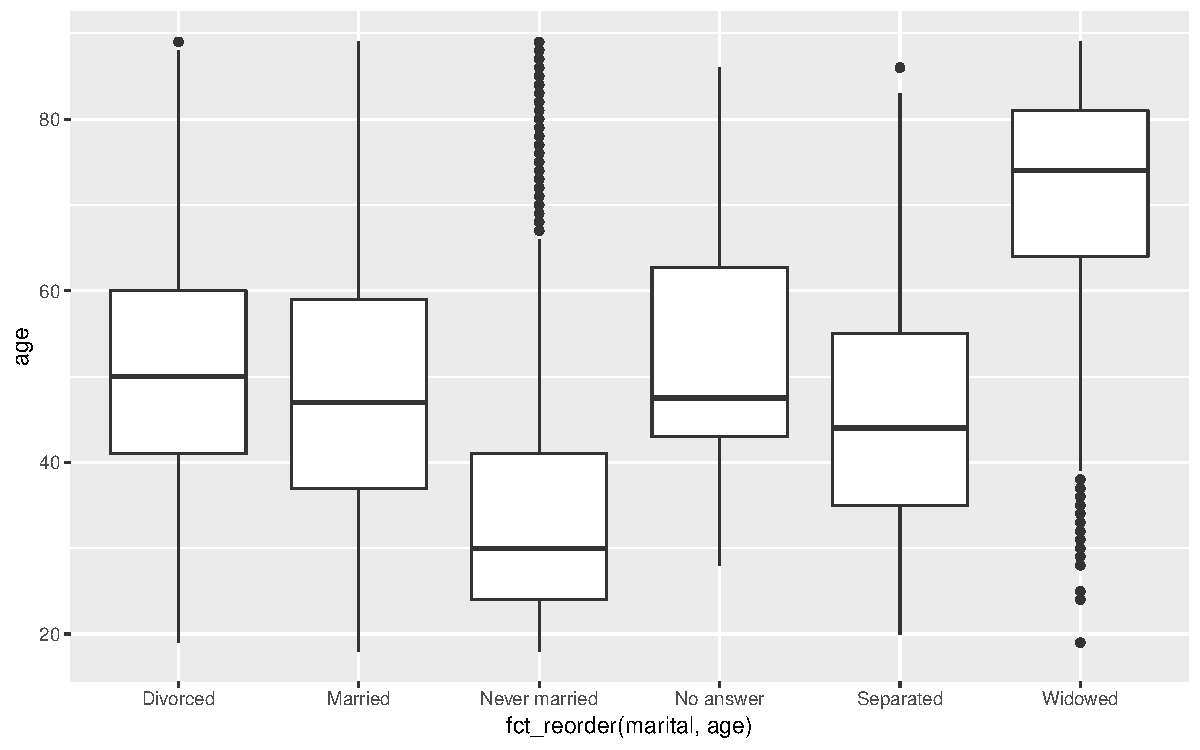
\includegraphics{cleaning_tutorial_files/figure-latex/unnamed-chunk-89-1}

Again, the results are not as we would expect. What's different compared
to the previous use with frequencies?

There are actually two differences.

\begin{enumerate}
\def\labelenumi{\arabic{enumi}.}
\tightlist
\item
  Before, we had a single frequency for each religion, making it easy to
  sort them.
\end{enumerate}

Now, for each marital status, we have many persons with different ages.
We need to summarize them in a single value, such as the mean or median.
This can be done by adding the .fun argument in factor reorder.

fct\_reorder(marital, age, .fun = median)

\begin{enumerate}
\def\labelenumi{\arabic{enumi}.}
\setcounter{enumi}{1}
\tightlist
\item
  Some persons don't have an age, but a missing value.
\end{enumerate}

Computing any function when there are missing values leads to a missing
value. We have to make sure that missing values are ignored. Any
argument we add to fct\_reorder after the .fun argument will be
considered as a argument to this function. Thus, the following will
correctly sort the marital variable

fct\_reorder(marital, age, .fun = median, na.rm = T)

Putting it to the test:

\begin{Shaded}
\begin{Highlighting}[]
\NormalTok{survey }\OperatorTok\StringTok{ }\KeywordTok{ggplot}\NormalTok{(}\KeywordTok{aes}\NormalTok{(}\KeywordTok{fct_reorder}\NormalTok{(marital, age, }
    \DataTypeTok{.fun =}\NormalTok{ median, }\DataTypeTok{na.rm =}\NormalTok{ T), age)) }\OperatorTok{+}\StringTok{ }\KeywordTok{geom_boxplot}\NormalTok{()}
\end{Highlighting}
\end{Shaded}

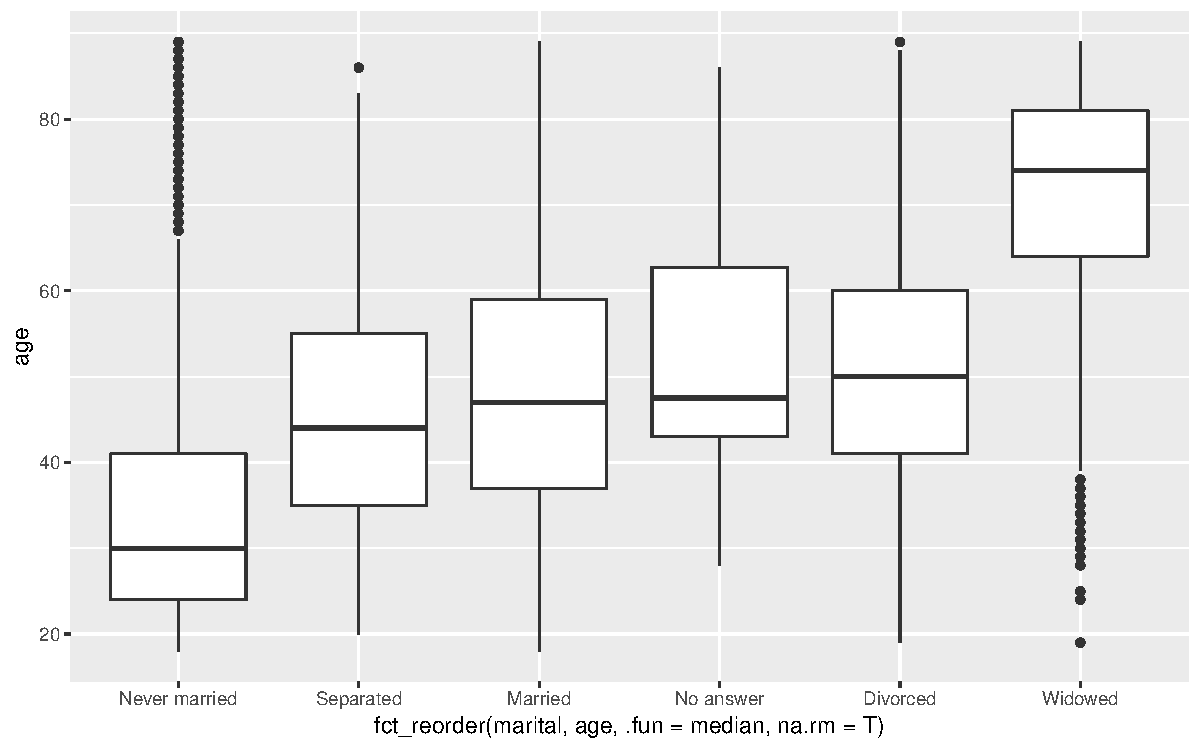
\includegraphics{cleaning_tutorial_files/figure-latex/unnamed-chunk-90-1}

This looks better. So, let's summarize once again.

\begin{itemize}
\tightlist
\item
  \texttt{fct\_infreq(f)}: reorder the levels of factor f from most to
  least frequent
\item
  \texttt{fct\_reorder}: reorder the levels of factor f according to
  variable x

  \begin{itemize}
  \tightlist
  \item
    \texttt{fct\_reorder(f,x)} when we are sure there is a single
    x-value for every f-level
  \item
    \texttt{fct\_reorder(f,x,\ .fun\ =\ summarize\_function)} when there
    can be more than one x-value for some f-level. The
    \texttt{summarize\_function} will be used to combine multiple
    values. This can be mean, median, sum, length, \ldots{} any function
    that returns a single value.
  \item
    If we need to give additional arguments to the summarize function,
    such as na.rm = T, we can do this as follows:
    \texttt{fct\_reorder(f,x,\ .fun\ =\ summarize\_function,\ na.rm\ =\ T)}.
  \end{itemize}
\item
  \texttt{fct\_rev(f)}: reverse the order of the levels of factor f
\end{itemize}

\chapter*{Background Material}\label{background-material-1}
\addcontentsline{toc}{chapter}{Background Material}

\begin{itemize}
\tightlist
\item
  More information on cleaning and transformation can be found in
  Prof.~dr. Depaire's Lecture Notes
\item
  More information on forcats can be read in Chapter 15 of
  \href{https://r4ds.had.co.nz/factors.html}{R for Data Science}
\end{itemize}



\end{document}
